\documentclass[UTF8,fontset=windows,zihao=5,a4paper]{ctexart}

% ---- 版心：中文期刊惯例，四周留白较宽
\usepackage{geometry}
\geometry{top=2.0cm,bottom=1.9cm,left=1.95cm,right=1.95cm,headsep=0.55cm,footskip=0.85cm}
\usepackage{xcolor}
\usepackage{graphicx}
\usepackage{booktabs}
\usepackage{longtable}
\usepackage{array}
\usepackage{ragged2e}
\usepackage{fancyhdr}
\usepackage{enumitem}
\usepackage{caption}
\usepackage{fancyvrb}
\usepackage{fvextra}
\usepackage[hidelinks]{hyperref}

\definecolor{ink}{HTML}{000000}
\definecolor{accent}{HTML}{8C2F00}
\definecolor{rule}{HTML}{9AA5B1}

% ---- 标题层级：黑体，编号与文字之间留一字空
\ctexset{
  section = {
    format = \zihao{4}\heiti\raggedright,
    beforeskip = 14pt plus 2pt minus 2pt,
    afterskip = 8pt plus 1pt minus 1pt,
  },
  subsection = {
    format = \zihao{5}\heiti\raggedright,
    beforeskip = 10pt plus 1pt minus 1pt,
    afterskip = 5pt plus 1pt,
  },
  subsubsection = {
    format = \zihao{5}\heiti\raggedright,
    beforeskip = 8pt plus 1pt,
    afterskip = 4pt,
  },
}

% ---- 正文：宋体五号，首行缩进两字，段间不空行
\setlength{\parindent}{2em}
\setlength{\parskip}{0pt}
\linespread{1.06}
\AtBeginDocument{\fontsize{8.7}{10.6}\selectfont}
\renewcommand{\arraystretch}{1.14}

\setlist[itemize]{leftmargin=2.2em,itemsep=1pt,topsep=3pt,parsep=0pt}
\setlist[enumerate]{leftmargin=2.4em,itemsep=1pt,topsep=3pt,parsep=0pt}

% 行内代码与正文视觉同号：等宽字体的 x 高度偏小，等比放大一档
\renewcommand{\texttt}[1]{{\ttfamily\fontsize{9.2}{11}\selectfont #1}}

% ---- 图表题注：中文期刊习惯，"图 1　题名"，居中，黑体小五
\DeclareCaptionFont{heifont}{\zihao{6}\heiti}
\captionsetup{font=heifont,labelsep=quad,justification=centering,skip=5pt}
\captionsetup[table]{position=top,skip=5pt}

% ---- 页眉页脚
\pagestyle{fancy}
\fancyhf{}
\renewcommand{\headrulewidth}{0.4pt}
\renewcommand{\headrule}{\hbox to\headwidth{\color{rule}\leaders\hrule height \headrulewidth\hfill}}
\fancyhead[C]{\zihao{6}\songti SciAgent：意图驱动的全流程科研助手}
\fancyfoot[C]{\zihao{6}\thepage}

% ---- 引文块：期刊通常用楷体缩进，不用彩色框
\newenvironment{aside}{\par\vspace{2pt}\begingroup\zihao{5}\kaishu
  \leftskip=2em\rightskip=2em\noindent\ignorespaces}{\par\endgroup\vspace{2pt}}

% ---- 圈号 ①② 与带圈字母：xeCJK 默认不把这两段交给中文字体，需显式指定
\xeCJKDeclareCharClass{CJK}{"2460 -> "24FF, "3200 -> "33FF}

\begin{document}
\thispagestyle{empty}
\begin{center}
\vspace*{2.2cm}
{\small\color{accent} 全国高校 AI 大模型创新应用挑战赛}\\[1.2cm]
{\Huge\bfseries SciAgent}\\[0.5cm]
{\LARGE 意图驱动的全流程科研助手}\\[1.0cm]
{\large 技 术 文 档}\\[2.2cm]
\begin{tabular}{@{}r@{\hspace{1.2em}}l@{}}
\end{tabular}
\end{center}
\vfill
\clearpage
\tableofcontents
\clearpage
<!-- cover -->

\subsubsection*{全国高校 AI 大模型创新应用挑战赛}
\section*{SciAgent}
\addcontentsline{toc}{section}{SciAgent}
\subsection*{意图驱动的全流程科研助手}
\addcontentsline{toc}{subsection}{意图驱动的全流程科研助手}
\subsubsection*{技术文档}
\begin{longtable}{@{}p{0.270\textwidth}p{0.690\textwidth}@{}}
\toprule
\multicolumn{1}{c}{\textbf{}} & \multicolumn{1}{c}{\textbf{}} \\
\midrule
\endfirsthead
\toprule
\multicolumn{1}{c}{\textbf{}} & \multicolumn{1}{c}{\textbf{}} \\
\midrule
\endhead
\bottomrule
\endfoot
\textbf{作品名称} & SciAgent · 科研小助手 \\
\textbf{赛项} & 智领科研·意图驱动：基于大模型与 Agent 架构的全流程科研助手构建 \\
\textbf{团队} & SciAgent Team · 西安交通大学 电子与信息学部 软件学院 \\
\textbf{仓库} & https://github.com/akawrzzby/sciagent \\
\textbf{在线演示} & https://finished-editing-shore-mrna.trycloudflare.com \\
\textbf{文档版本} & v1.0 · 2026-11 \\
\end{longtable}

\subsection*{摘要}
\addcontentsline{toc}{subsection}{摘要}
本文报告 SciAgent 的设计与实现。SciAgent 面向科研文献的阅读与写作，将检索、精读、对比、综述与写作组织为一条可溯源的流水线。

系统由三个子系统构成。多模态解析引擎采用版式感知的解析策略，还原双栏阅读顺序、章节树、表格、图、公式与结构化参考文献；对无文本层的扫描件，改由多模态模型逐页转写。Agent 编排采用取证与生成分离的两阶段结构：第一阶段产出携带字符区间的证据集合，第二阶段仅依据该集合生成正文，两阶段之间以证据为唯一接口。图论挖掘在引用图上计算 PageRank、介数中心性、k-core 与 HITS，据此区分基石文献与衍生文献，并生成领域综述与研究机会。

在赛题提供的 39 篇测试集上，系统对 \texttt{1706.03762v1.pdf} 的版式解析耗时 4.2 秒，含公式转写的端到端耗时为 71.7 秒；8 位作者、26 个章节节点与 71 条结构化参考文献均正确还原。稠密检索通道对语义相近文本的余弦相似度为 0.89，对语义无关文本为 0.38；重排通道对切题段落给出 +0.92，对离题段落给出 +0.00。

全文组织如下：第 1 节说明问题背景与系统定位，第 2 节给出功能与非功能需求，第 3 节描述架构设计，第 4 节论述 AI 技术的选型理由、集成方式与优化策略，第 5 节说明各模块的实现，第 6 节报告测试与部署结果，第 7 节总结全文，第 8 节单列技术创新点与应用创新点。

\subsection*{1. 项目概述}
\addcontentsline{toc}{subsection}{1. 项目概述}
\subsubsection*{1.1 问题背景}
科研文献的机器化利用受制于五类问题。

其一，PDF 并非结构化文本。学术 PDF 普遍采用双栏排版，并含跨栏图表、数学公式与脚注；直接提取所得到的字符序列在阅读顺序上已经错乱，纯图像扫描件更不含任何文本层。若解析阶段不能恢复版面结构，后续的分块、检索与问答均失去可靠基础。

其二，生成内容的可信度不足。通用语言模型在陈述论文细节时存在虚构现象，包括杜撰参考文献、混淆作者归属，以及将一篇论文的结论归入另一篇名下。OpenScholar 的统计给出了量级：在带引用生成任务中，GPT-4o 的引用幻觉率为 78\% 至 90\%，即十条引用中至少有八条无法核实。该现象并非孤例：PubMed Central 上被判定为伪造的引用比例由 2023 年的 1/2828 上升至 2025 年的 1/458，2026 年前七周进一步升至 1/277；GPTZero 在 NeurIPS 2025 录用的 51 篇论文中检出 100 条幻觉引用；另一项统计显示，仅约 26.5\% 的 AI 生成引用完全正确。检索所解决的是材料获取问题，引用可溯源与矛盾可发现属于另外两项能力，本文将其分别实现。

其三，阅读工具彼此割裂。PDF 阅读器忠实于版式却不理解语义，翻译工具能翻译却丢失指代关系，文献管理软件能收藏却不支持提问。一篇三十页的论文往往需要在四个工具之间往复切换方能读通。

其四，方向判断缺乏依据。阅读二十篇论文可以复述各自的结论，却难以回答该方向尚存哪些空白、哪些问题被反复提出而未获解决。

其五，写作环节缺少支撑。论文框架、系统架构图与数据表格均需从空白文档起笔；其中的参考文献尤易出错，凭记忆写出的条目常有一半查无此文。

\subsubsection*{1.2 系统定位与目标}
SciAgent 定位为面向科研文献的可溯源处理流水线，其设计遵循三项原则。

\begin{longtable}{@{}p{0.227\textwidth}p{0.733\textwidth}@{}}
\toprule
\multicolumn{1}{c}{\textbf{原则}} & \multicolumn{1}{c}{\textbf{含义}} \\
\midrule
\endfirsthead
\toprule
\multicolumn{1}{c}{\textbf{原则}} & \multicolumn{1}{c}{\textbf{含义}} \\
\midrule
\endhead
\bottomrule
\endfoot
证据优先 & 每一项结论均须指回原文的字符区间；无法指回者不予陈述。 \\
结构优先 & 标题、表格、公式与参考文献分别建模，不做无结构的文本拼接。 \\
可降级 & 稠密检索通道失效时退化为 BM25；语言模型超时则返回明确错误，不做静默失败。 \\
\end{longtable}

上述原则对应三项可度量的目标。

\begin{itemize}
\item 解析准确：对测试集内的标准论文，标题层级、作者、表格与参考文献字段全部正确；对扫描件，能够产出可检索的正文。
\item 回答可信：全部回答携带可点击的溯源锚点，包含文献标识、页码与字符区间；证据不足时明确拒答。
\item 闭环完整：从文献入库到综述、框架与图表生成，全流程在系统内完成。
\end{itemize}

\subsubsection*{1.3 赛题要求映射}
\begin{longtable}{@{}p{0.204\textwidth}p{0.363\textwidth}p{0.392\textwidth}@{}}
\toprule
\multicolumn{1}{c}{\textbf{赛题模块}} & \multicolumn{1}{c}{\textbf{系统对应实现}} & \multicolumn{1}{c}{\textbf{关键支撑技术}} \\
\midrule
\endfirsthead
\toprule
\multicolumn{1}{c}{\textbf{赛题模块}} & \multicolumn{1}{c}{\textbf{系统对应实现}} & \multicolumn{1}{c}{\textbf{关键支撑技术}} \\
\midrule
\endhead
\bottomrule
\endfoot
① 多模态细粒度文档解析 & \texttt{backend/app/parsing/} & 版式分析、栏检测、标题树推断、VLM OCR、语义去重 \\
② 意图驱动检索与抗幻觉 & \texttt{backend/app/rag/}、\texttt{backend/app/agents/} & 稀疏检索、稠密检索、排名融合与交叉编码精排；证据绑定与引用真实性校验 \\
③ 版式阅读与中英联动 & \texttt{frontend/src/pages/Reader.tsx} & 双栏渲染、引用双向跳转、段落对齐滚动 \\
④ arXiv 检索与追踪 & \texttt{backend/app/tools/sources.py} & arXiv API、GitHub Search、Function Calling 闭环 \\
⑤ 文献图谱与基石挖掘 & \texttt{backend/app/graph/} & PageRank、Betweenness、k-core、HITS \\
⑥ 论文写作辅助 & \texttt{backend/app/api/routers/writing.py}、\texttt{tools/viz.py} & 框架生成、TikZ 与 Mermaid 及 Graphviz 绘图、由 CSV 数据生成图表与图注 \\
\end{longtable}

\subsubsection*{1.4 对照评分标准的自评}
赛题说明书的评分标准包含五个维度：AI 技术深度 35\%、创新性 15\%、产品功能和工程质量 30\%、用户体验 10\%、实用性 10\%。本人在赛题官方材料中未查到细分到考察点的权重，故下表为本人所作的拆解：将五个维度展开为 18 项可核验的考察点，并给出其在系统中的实现位置与对应证据。

\begin{longtable}{@{}p{0.166\textwidth}p{0.293\textwidth}p{0.501\textwidth}@{}}
\toprule
\multicolumn{1}{c}{\textbf{考察点}} & \multicolumn{1}{c}{\textbf{实现位置}} & \multicolumn{1}{c}{\textbf{可核验证据}} \\
\midrule
\endfirsthead
\toprule
\multicolumn{1}{c}{\textbf{考察点}} & \multicolumn{1}{c}{\textbf{实现位置}} & \multicolumn{1}{c}{\textbf{可核验证据}} \\
\midrule
\endhead
\bottomrule
\endfoot
Agent 架构与任务规划 & \texttt{agents/orchestrator.py} & 意图路由、任务规划、工具取证、带证据生成与自反馈五个环节均在界面的思考面板中逐步呈现；事件类型见 §9.1 \\
抗幻觉检索与溯源 & \texttt{rag/retriever.py}、\texttt{rag/sparse.py}、\texttt{rag/embeddings.py}、\texttt{llm/guardrails.py} & 混合检索与交叉编码精排；每条引用携带分块标识、页码与字符区间，可在界面打开原文；引用按支持、对照、提及三类标注；三轮评测的忠实度为 0.8034，可溯源率为 1.0000；库外对照题三次均拒答且无编造，见 §6.3.4 与 §6.3.5 \\
多模态与细粒度解析 & \texttt{parsing/} & 扫描件 15 页经识别后还原 26 个章节节点；541 页书籍耗时 149.4 秒，产出 1254 个章节节点与 131 万字符，见 §6.4 与 T24 \\
工具调用与集成 & \texttt{tools/} & 工具由模型自主选择，调用过程在轨迹中逐条可见；经 arXiv 下载入库的论文可被检索命中 \\
提示词与护栏 & \texttt{llm/prompts.py}、\texttt{llm/guardrails.py} & 六层护栏各有单元测试，见 T18 至 T22 与 T35 至 T37；第六层源于一处真实缺陷，见 §4.10 \\
图谱算法 & \texttt{graph/} & 四项中心性指标联合判定基石文献，见 T16；15 篇库上矛盾检测仅保留 1 条真实冲突，即 BLEU 41.0 与 41.8，误报为零，见 T33 与 T42 \\
技术方案与检索创新 & 语义去重、版本差异比对、元数据感知检索、按断言级的引用修复 & v1 与 v7 判为同一论文并给出保留建议；作者块重排分由 0.058 升至 0.719；元数据感知检索的 top-5 命中率由 0.9286 升至 1.0000，见 §4.5 与 §6.3.6 \\
科研交互模式 & \texttt{Reader.tsx} & 标题树定位、引用双向跳转、中英对照同步滚动 \\
代码质量与架构 & 前端 TypeScript，后端 Python & 227 个用例通过；静态作用域检查已固化为测试，见 T29 \\
可复现性与部署 & 容器编排文件、镜像定义、环境变量模板 & 以单条命令启动全栈；本地模型经兼容端点接入 \\
渲染性能与内存 & \texttt{rag/embeddings.py}、\texttt{parsing/}、\texttt{graph/} & 在 64 线程下，编码吞吐由每秒 7.2 篇升至 99.7 篇，约为 13.8 倍；向量索引按论文文件化并以内存映射方式加载 \\
科研场景契合度 & 六个工作台 & 覆盖检索、精读、对比与写作四个环节，见 §5 \\
功能闭环与用例通过率 & 四类指定用例 & 版本去重、扫描件识别、541 页书籍解析、由 CSV 生成图表，见 §6.2 与 §6.4 \\
界面设计与可视化 & \texttt{GraphWorkbench.tsx}、\texttt{WritingWorkbench.tsx} & 图谱三种边视图、基石与衍生双视图、矛盾检测面板均经浏览器实测 \\
联动阅读与前端体验 & \texttt{Reader.tsx} & 标题树可定位至 \texttt{3.2.2 Multi-Head Attention}；引用双向跳转 \\
思考过程与流式渲染 & 事件流与前端思考面板 & 令牌级流式输出；思考过程可视化；自反馈补检索单独成条 \\
学术赋能价值 & 整条流水线 & 见 §5 与 §7 \\
开源与复现 & 仓库结构、环境变量模板、容器编排、评测脚本 & 评测脚本可复跑全部数字 \\
\end{longtable}

\subsection*{2. 需求分析}
\addcontentsline{toc}{subsection}{2. 需求分析}
\subsubsection*{2.1 功能需求}
本人将赛题提出的功能要求分解为可验收的条目，按 F1 至 F6 六组编号。

\textbf{F1 文档解析}

\begin{itemize}
\item F1.1 解析标题树，保留层级与编号，须支持三级以上编号。
\item F1.2 还原双栏 PDF 的正确阅读顺序。
\item F1.3 抽取表格，同时输出 Markdown 与 CSV 两种格式。
\item F1.4 抽取图片及其图注。
\item F1.5 抽取行内公式与块级公式。
\item F1.6 将参考文献解析为结构化字段，含作者、标题、年份、会议、DOI 与 arXiv 编号。
\item F1.7 对无文本层的 PDF 执行识别，识别结果参与后续检索。
\item F1.8 识别同一论文的不同版本，并给出保留建议与版本差异。
\end{itemize}

\textbf{F2 检索与问答}

\begin{itemize}
\item F2.1 混合检索：稀疏与稠密双通道，经 RRF 融合后由 cross-encoder 精排。
\item F2.2 答案携带溯源锚点，可定位到具体文献、页码与字符区间。
\item F2.3 Agent 能够自主拆解任务并调用外部工具，包括 arXiv、GitHub、本地检索与绘图。
\item F2.4 证据不足时拒答。
\item F2.5 流式输出，思考过程可视化。
\end{itemize}

\textbf{F3 阅读器}

\begin{itemize}
\item F3.1 标题树定位，点击跳转至对应页面。
\item F3.2 原文版式高保真还原。
\item F3.3 中英双栏对照，滚动同步。
\item F3.4 正文引用标记与参考文献条目双向跳转。
\end{itemize}

\textbf{F4 检索与推荐}

\begin{itemize}
\item F4.1 arXiv 关键词检索与分类追踪。
\item F4.2 下载 PDF 后自动解析入库。
\item F4.3 基于文献库的推荐，优先推荐有公开代码的可复现工作。
\item F4.4 用户反馈参与排序。
\end{itemize}

\textbf{F5 图谱}

\begin{itemize}
\item F5.1 构建库内引用有向图。
\item F5.2 计算多种中心性指标并可视化。
\item F5.3 判定基石节点。
\item F5.4 自动生成领域综述。
\item F5.5 挖掘后续研究机会。
\end{itemize}

\textbf{F6 写作}

\begin{itemize}
\item F6.1 生成论文框架，含标题、摘要、引言、相关工作、方法与实验。
\item F6.2 生成的参考文献须为库内真实存在者，否则拦截。
\item F6.3 生成 TikZ、Mermaid 与 Graphviz 架构图。
\item F6.4 由 CSV 数据生成学术图表与图注。
\end{itemize}

\subsubsection*{2.2 非功能需求}
\begin{longtable}{@{}p{0.148\textwidth}p{0.297\textwidth}p{0.515\textwidth}@{}}
\toprule
\multicolumn{1}{c}{\textbf{维度}} & \multicolumn{1}{c}{\textbf{指标}} & \multicolumn{1}{c}{\textbf{设计对策}} \\
\midrule
\endfirsthead
\toprule
\multicolumn{1}{c}{\textbf{维度}} & \multicolumn{1}{c}{\textbf{指标}} & \multicolumn{1}{c}{\textbf{设计对策}} \\
\midrule
\endhead
\bottomrule
\endfoot
解析性能 & 标准论文的解析时间小于 5 秒 & 版式分析在处理器上完成；按页并行；仅对检测为扫描件的文档执行识别 \\
长文档 & 500 页以上不发生内存溢出 & 按页流式处理；向量按篇以内存映射方式存放；查询期仅载入参与检索的论文 \\
流式体验 & 首令牌延迟小于 3 秒 & 采用两阶段架构，取证结果先行返回；事件流全链路关闭缓冲 \\
鲁棒性 & 单通道故障不影响整体可用性 & 稠密检索、重排与语言模型分别降级；后台任务异常隔离 \\
可复现 & 以单条命令启动全栈 & 提供容器编排文件与环境变量模板 \\
安全 & 密钥不外泄 & 密钥经环境变量注入；配置文件不纳入版本库；仓库内无任何密钥 \\
可审计 & 每次模型调用可追溯 & 系统提示、用户提示、工具参数、耗时与令牌数全部落盘 \\
\end{longtable}

\subsubsection*{2.3 竞品与现有方案对比}
本节选取赛题相关的八项同类工作，说明本文与它们在设计取舍上的异同，见表 2；各工作的完整出处见 §9.4。

\begin{longtable}{@{}p{0.324\textwidth}p{0.636\textwidth}@{}}
\toprule
\multicolumn{1}{c}{\textbf{方案}} & \multicolumn{1}{c}{\textbf{本文的借鉴与差异}} \\
\midrule
\endfirsthead
\toprule
\multicolumn{1}{c}{\textbf{方案}} & \multicolumn{1}{c}{\textbf{本文的借鉴与差异}} \\
\midrule
\endhead
\bottomrule
\endfoot
PaperQA2 [20] & 借鉴其元数据感知检索与矛盾检测思路。差异在于 ContraCrow 依赖专门训练的矛盾检测器与大规模语料；本文因库内互引仅 14 条、训练素材不足，改走规则化路线 \\
OpenScholar [21] & 借鉴其自反馈循环与引用须可核验的设计。差异在于其规模不可复现；本文在 15 篇的库上将可核验性落实为可点击的字符区间锚点 \\
STORM [22] & 借鉴其先大纲后写作的组织方式。本文未引入多智能体角色扮演层，理由见 §8.3 \\
Agent Laboratory [23] & 借鉴其反思环节。该工作同时披露语言模型评审存在系统性高估：其自评为 6.1/10，人类评审为 3.8/10。本文因此不以模型自评作为效果证据 \\
Docling 与 PyMuPDF-Layout [26][27] & 在 DocLayNet 上 PyMuPDF-Layout 的 F1 为 0.8356，Docling 为 0.8102；前者参数量 1.8M，后者 20M，且前者无需 GPU。本文的选型依据即此组实测 \\
Scite、Elicit、Consensus [28] & 借鉴其引用三分类的标签体系。本文在三分类之上增加矛盾检测，判定过程全部可解释 \\
Connected Papers [29] & 借鉴其共引与共参考两种相似关系。本文将其实现为图谱的可切换边视图，而非独立站点 \\
本文工作 & — \\
\end{longtable}

就解析深度而言，Docling 与 PyMuPDF-Layout 面向版面元素识别，其表格结构化率虽高，但不产出结构化的参考文献与章节树，也不解决图与公式的版面归属；本文的解析目标是全要素结构，即标题、作者、摘要、章节树、表格、图、公式与参考文献各自建模。

就引用可溯源而言，PaperQA2 与 STORM 提供页级引用，Scite 一类工具提供引用原句与立场标签，OpenScholar 虽带引用但报告的幻觉率为 78\% 至 90\%。本文的锚点细至字符区间，即记录文献标识、页码、章节与正文起止位置，读者可据此定位到具体句子。

就矛盾检测而言，PaperQA2 的 ContraCrow 报告每篇 2.34±1.99 条矛盾、其中 70\% 经专家验证，但其检测器需专门训练。本文以三条规则实现数值冲突与结论冲突的判定：同指标、同任务上下文、取值不同；规则化实现的可解释性更强，代价是召回受限于规则的覆盖范围。在 15 篇的库上，该模块仅保留 1 条真实冲突并将误报压至零，这一取舍与上一段的判断一致。

上述比较的着眼点并非系统能否阅读文献，而在于其结论能否被证明。可证明性以字符为单位，每条引用指向具体位置，而非仅注明参考了某篇论文；可解释性贯穿全链路，引用立场、矛盾判定与检索排序的元数据加权均附判定依据；可举证性以数字呈现，§6.3 的三个指标在固定的 15 篇文献库上产出，并附可复跑脚本。

\subsection*{3. 系统架构设计}
\addcontentsline{toc}{subsection}{3. 系统架构设计}
\subsubsection*{3.1 总体架构}
\begin{figure}[htbp]
\centering
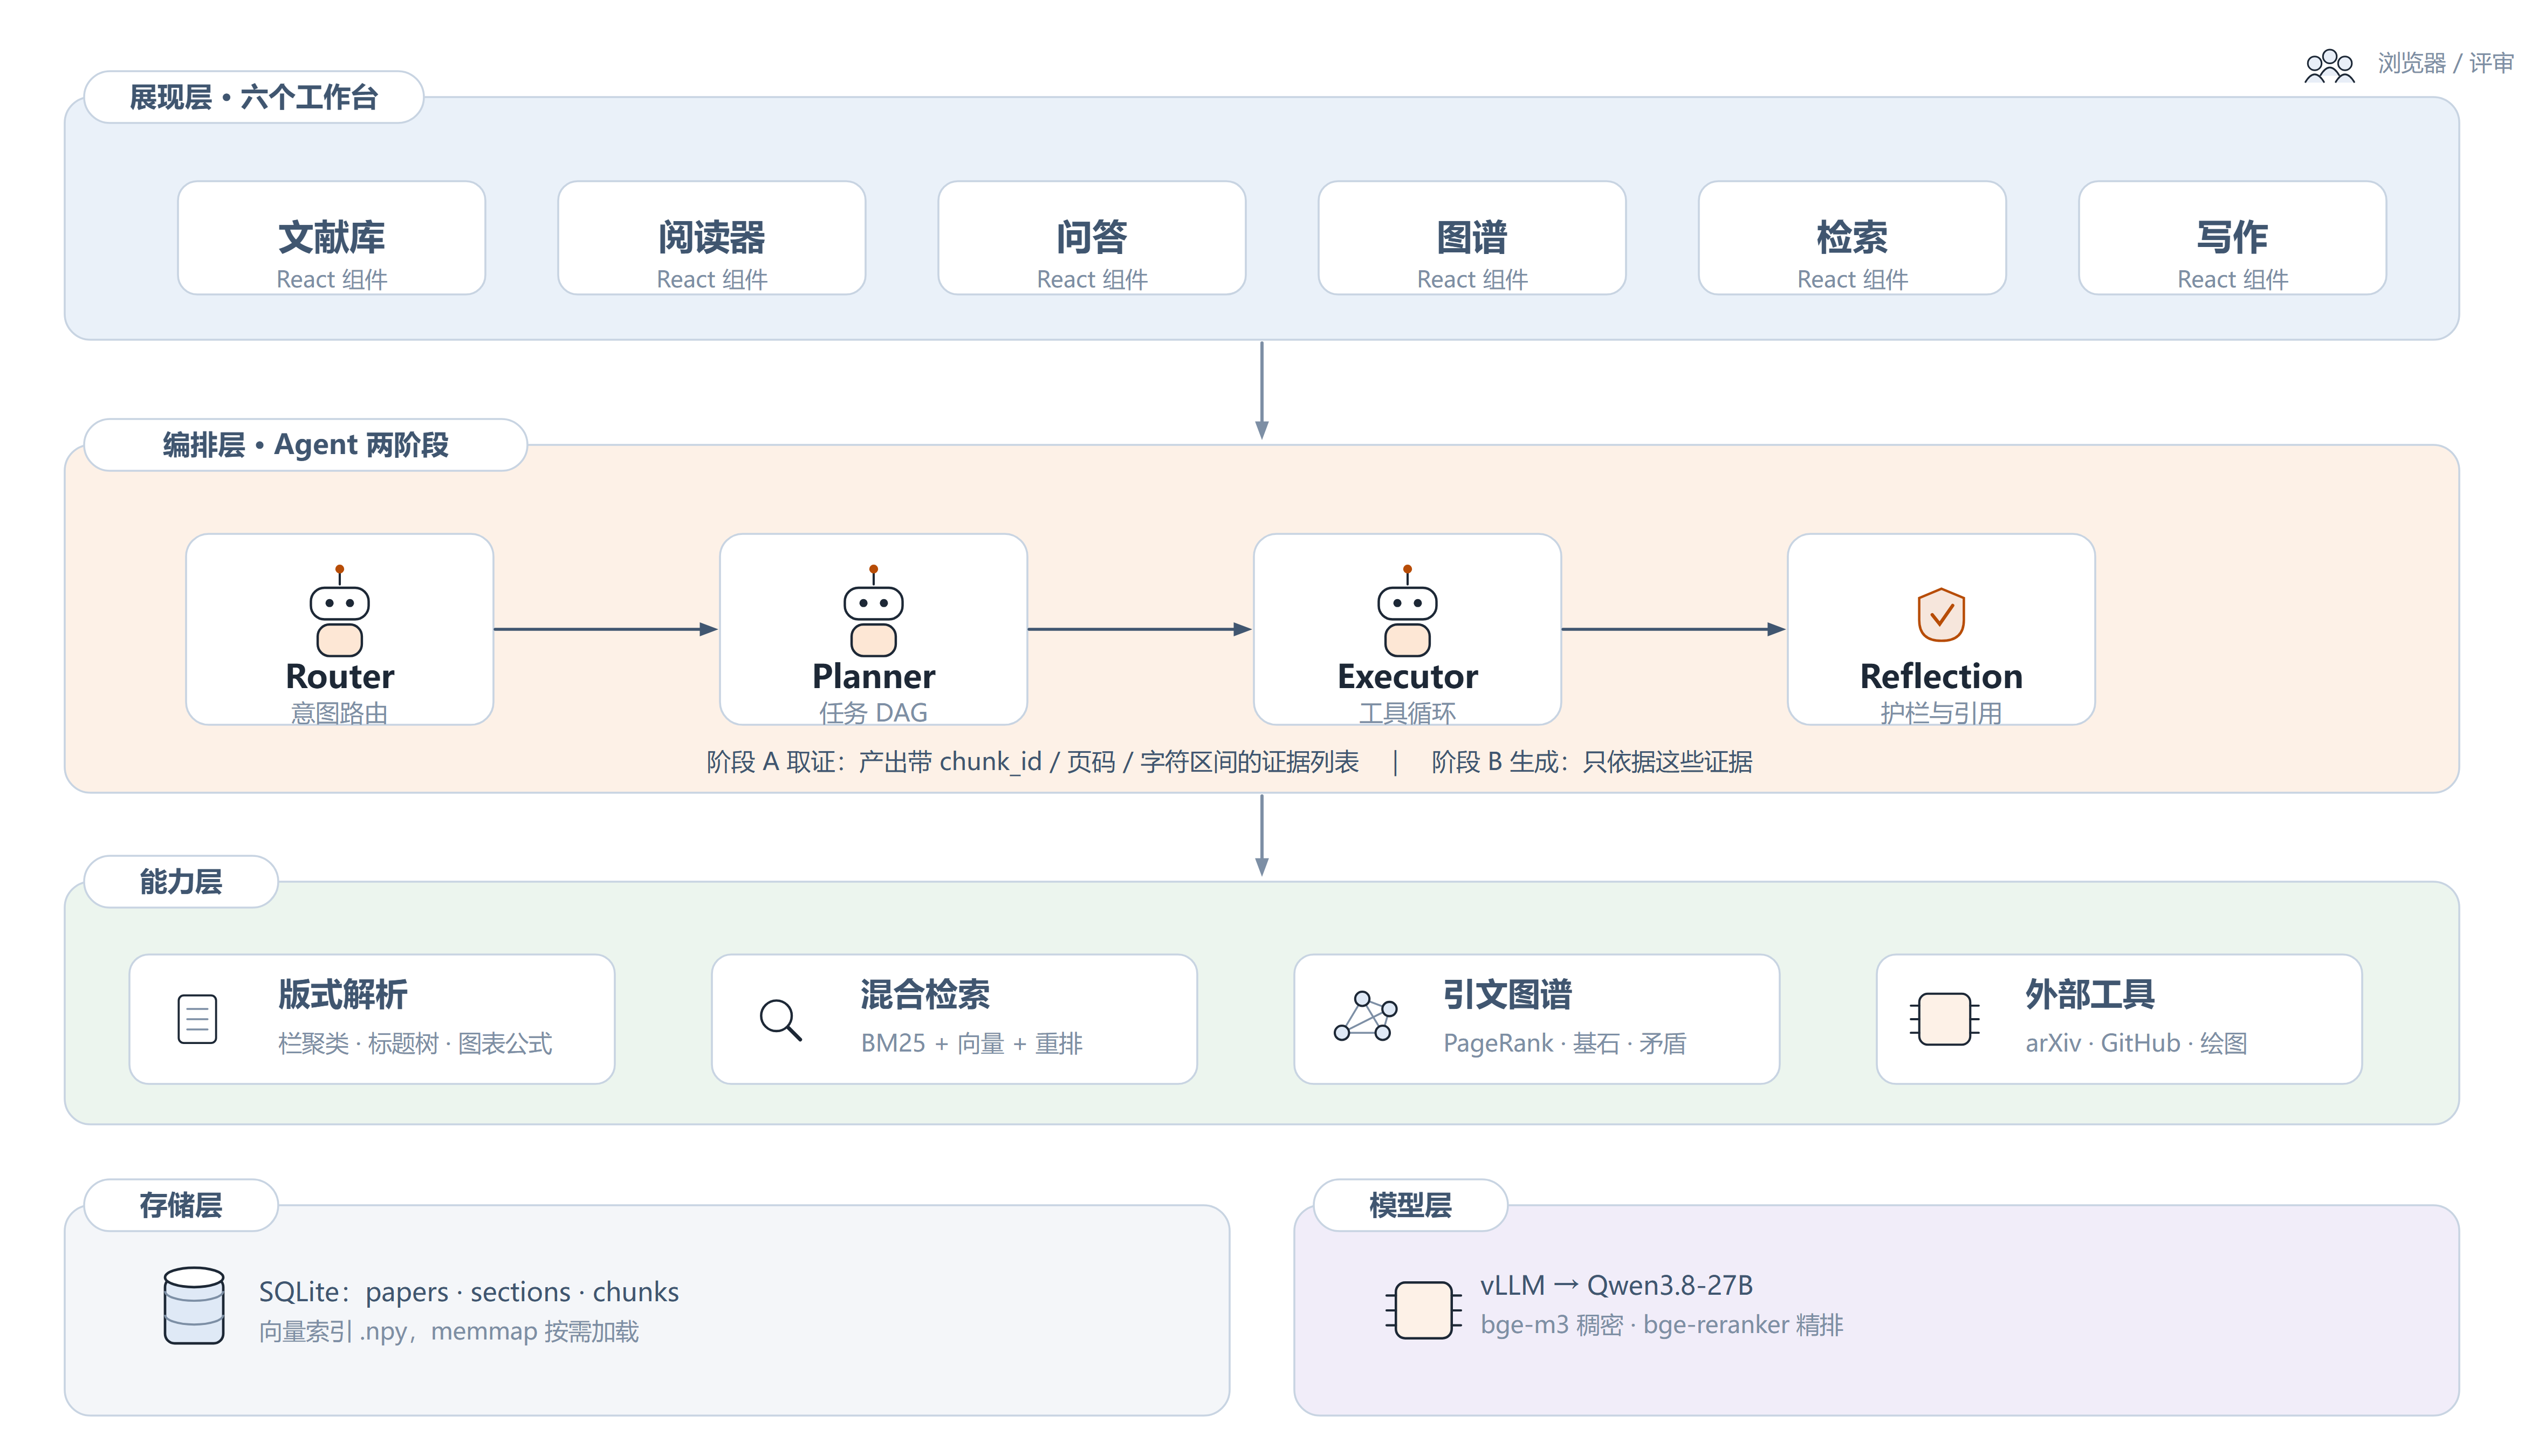
\includegraphics[width=0.88\textwidth]{figures/fig-arch.png}
\caption{系统分层架构。六个工作台共用同一套编排层与能力层，存储与模型居于底层}
\end{figure}

系统自下而上分为模型层、存储层、能力层、编排层与展现层，每一层仅依赖其下一层。展现层经 \texttt{/api} 接口与 SSE 事件流访问编排层；编排层调用能力层的纯函数；能力层读写存储，并向下使用模型。

此种分层的主要目的是使各层可独立测试。解析器不依赖 HTTP 服务即可运行，检索器不依赖语言模型在线即可运行；稠密通道不可用时，检索退化为 BM25，其余功能不受影响。

\subsubsection*{3.2 分层职责}
\begin{longtable}{@{}p{0.121\textwidth}p{0.463\textwidth}p{0.376\textwidth}@{}}
\toprule
\multicolumn{1}{c}{\textbf{层}} & \multicolumn{1}{c}{\textbf{模块}} & \multicolumn{1}{c}{\textbf{职责}} \\
\midrule
\endfirsthead
\toprule
\multicolumn{1}{c}{\textbf{层}} & \multicolumn{1}{c}{\textbf{模块}} & \multicolumn{1}{c}{\textbf{职责}} \\
\midrule
\endhead
\bottomrule
\endfoot
展现层 & \texttt{frontend/src/pages/*} & 六个工作台；仅依赖类型化客户端与 SSE 事件流 \\
编排层 & \texttt{app/agents/orchestrator.py}、\texttt{app/tools/registry.py} & 意图路由、任务规划、工具循环与结果反思 \\
能力层 & \texttt{app/parsing/}、\texttt{app/rag/}、\texttt{app/graph/}、\texttt{app/tools/} & 纯函数式能力，不依赖 HTTP \\
存储层 & \texttt{app/storage/} & 异步 ORM 与 SQLite 存储；向量索引以文件存放 \\
接入层 & \texttt{app/api/routers/} & 路由层，仅做参数校验与结果封装 \\
模型层 & \texttt{app/llm/client.py}、\texttt{app/rag/embeddings.py} & OpenAI 兼容客户端，以及编码器与重排器的封装 \\
\end{longtable}

解耦的关键在于两条约束：能力层不感知 Agent，Agent 不感知 HTTP。检索模块既可由检索工作台的接口直接调用，亦可由编排层作为工具调用，同一份检索逻辑对应两种入口，无需重复实现。

\subsubsection*{3.3 Agent 编排架构}
ReAct 范式将检索与生成纳入同一循环：模型思考、选择工具、观察结果、再次思考，直至自认为证据充分方开始撰写。该范式在科研场景下存在三方面问题。其一，工具调用与正文生成混在同一数据流中，界面无法区分系统处于取证阶段还是撰写阶段；其二，令牌流向不可控；其三，工具调用一旦失败，已生成的部分正文即被浪费。

针对上述问题，本文采用取证与生成分离的两阶段结构，如图 3-2 所示。

\begin{figure}[htbp]
\centering
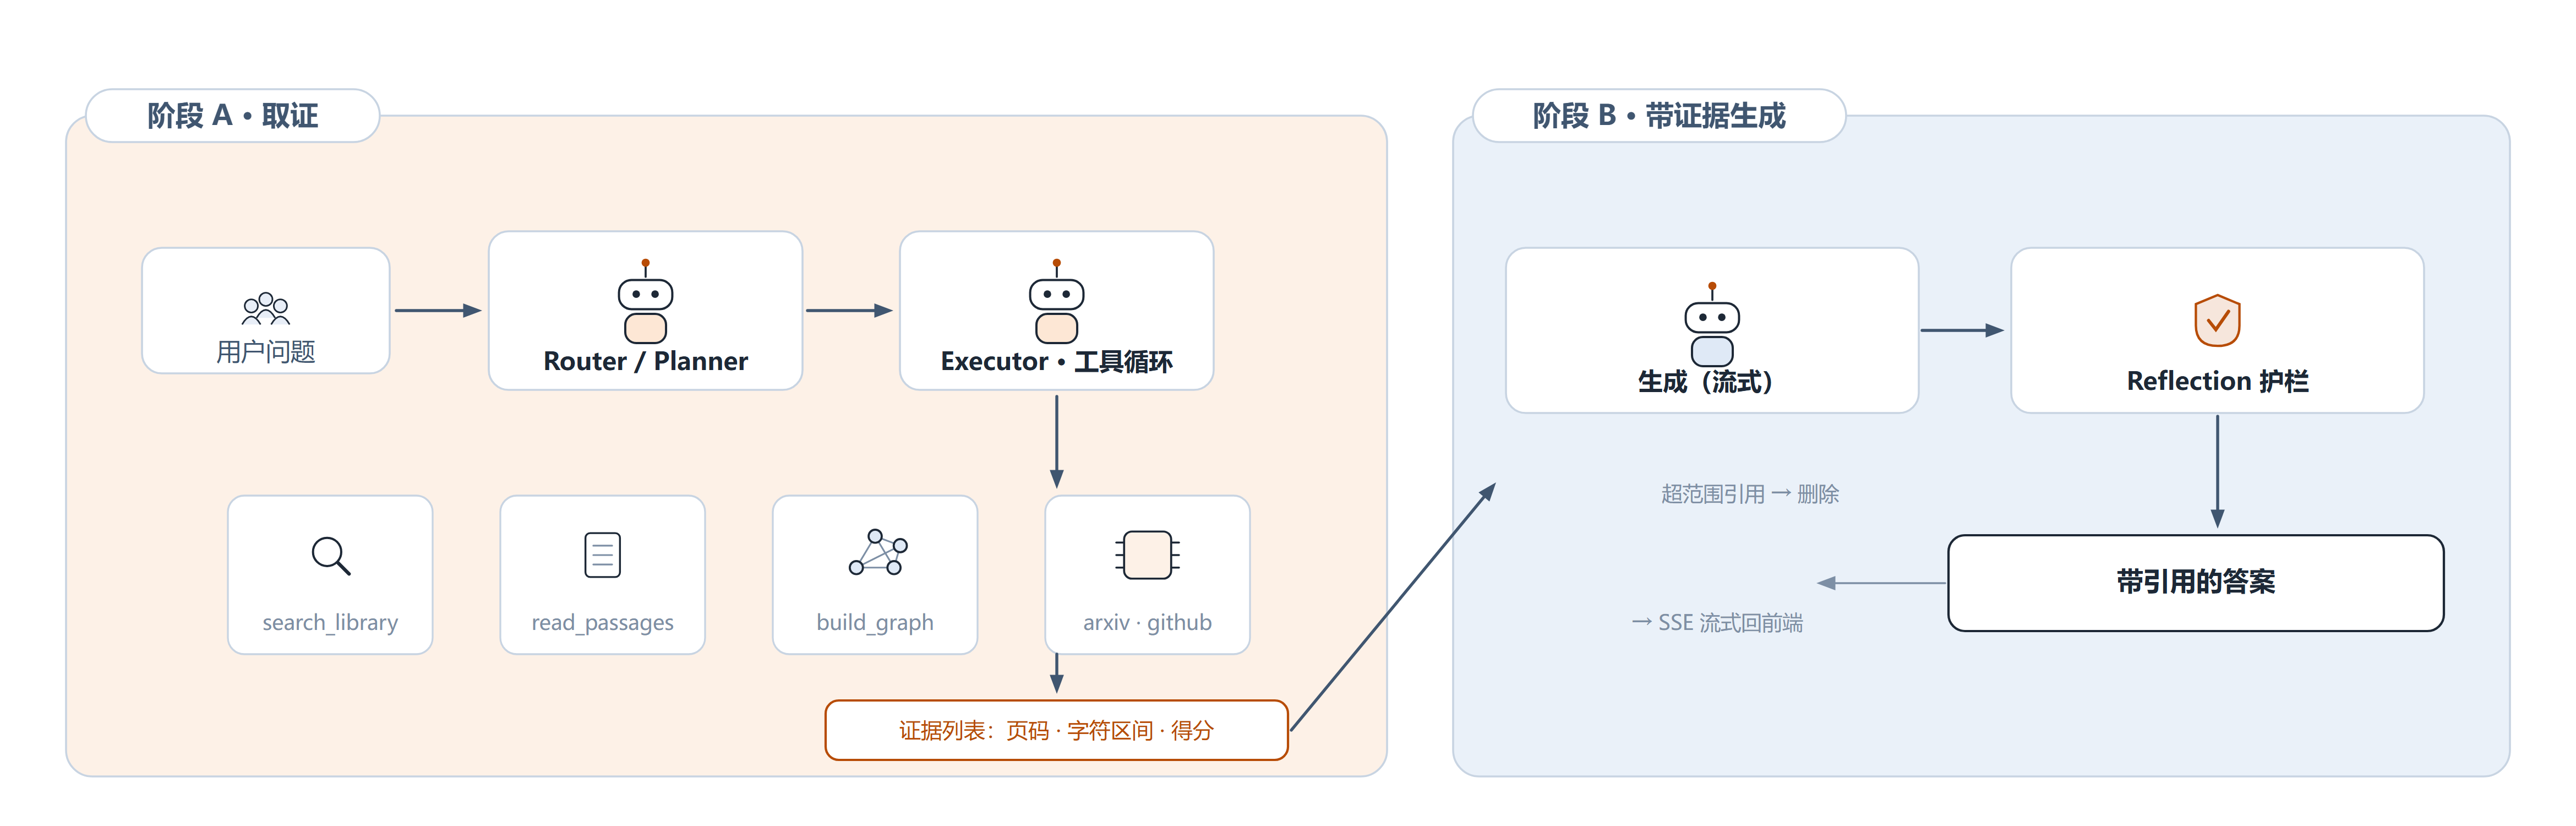
\includegraphics[width=0.88\textwidth]{figures/fig-agent.png}
\caption{两阶段 Agent 编排。阶段 A 负责取证，阶段 B 仅依据证据生成}
\end{figure}

阶段 A 为取证阶段，产出结构化的证据列表，每条记录包含文献标识、文献标题、页码、字符区间、原文片段、检索得分与来源通道。该列表在界面的思考过程面板中逐条呈现，使用者可据此判断结论依据了哪几段原文。

阶段 B 为生成阶段。其系统提示中仅包含上述证据，并显式限定引用编号的取值范围。生成完成后，反思阶段再行两项校验：

\begin{itemize}
\item 证据绑定：以正则扫描答案中的引用编号，凡不在证据集合内者一律删除，并将该答案标记为部分无据。
\item 引用真实性：写作助手生成的参考文献与库内文献做标题模糊匹配以及 arXiv 编号与 DOI 精确匹配，不匹配者进入已拦截列表，在界面中单独呈现。
\end{itemize}

两项校验的作用在于，即使模型试图陈述无依据的结论，其引用标记亦会被移除，界面同时给出被移除的数量。此处的取舍是宁可显式暴露失败，也不静默返回一个看似完整的答案。

\subsubsection*{3.4 数据流与时序}
图 3-3 给出一次跨文献问答的完整时序。

\begin{figure}[htbp]
\centering
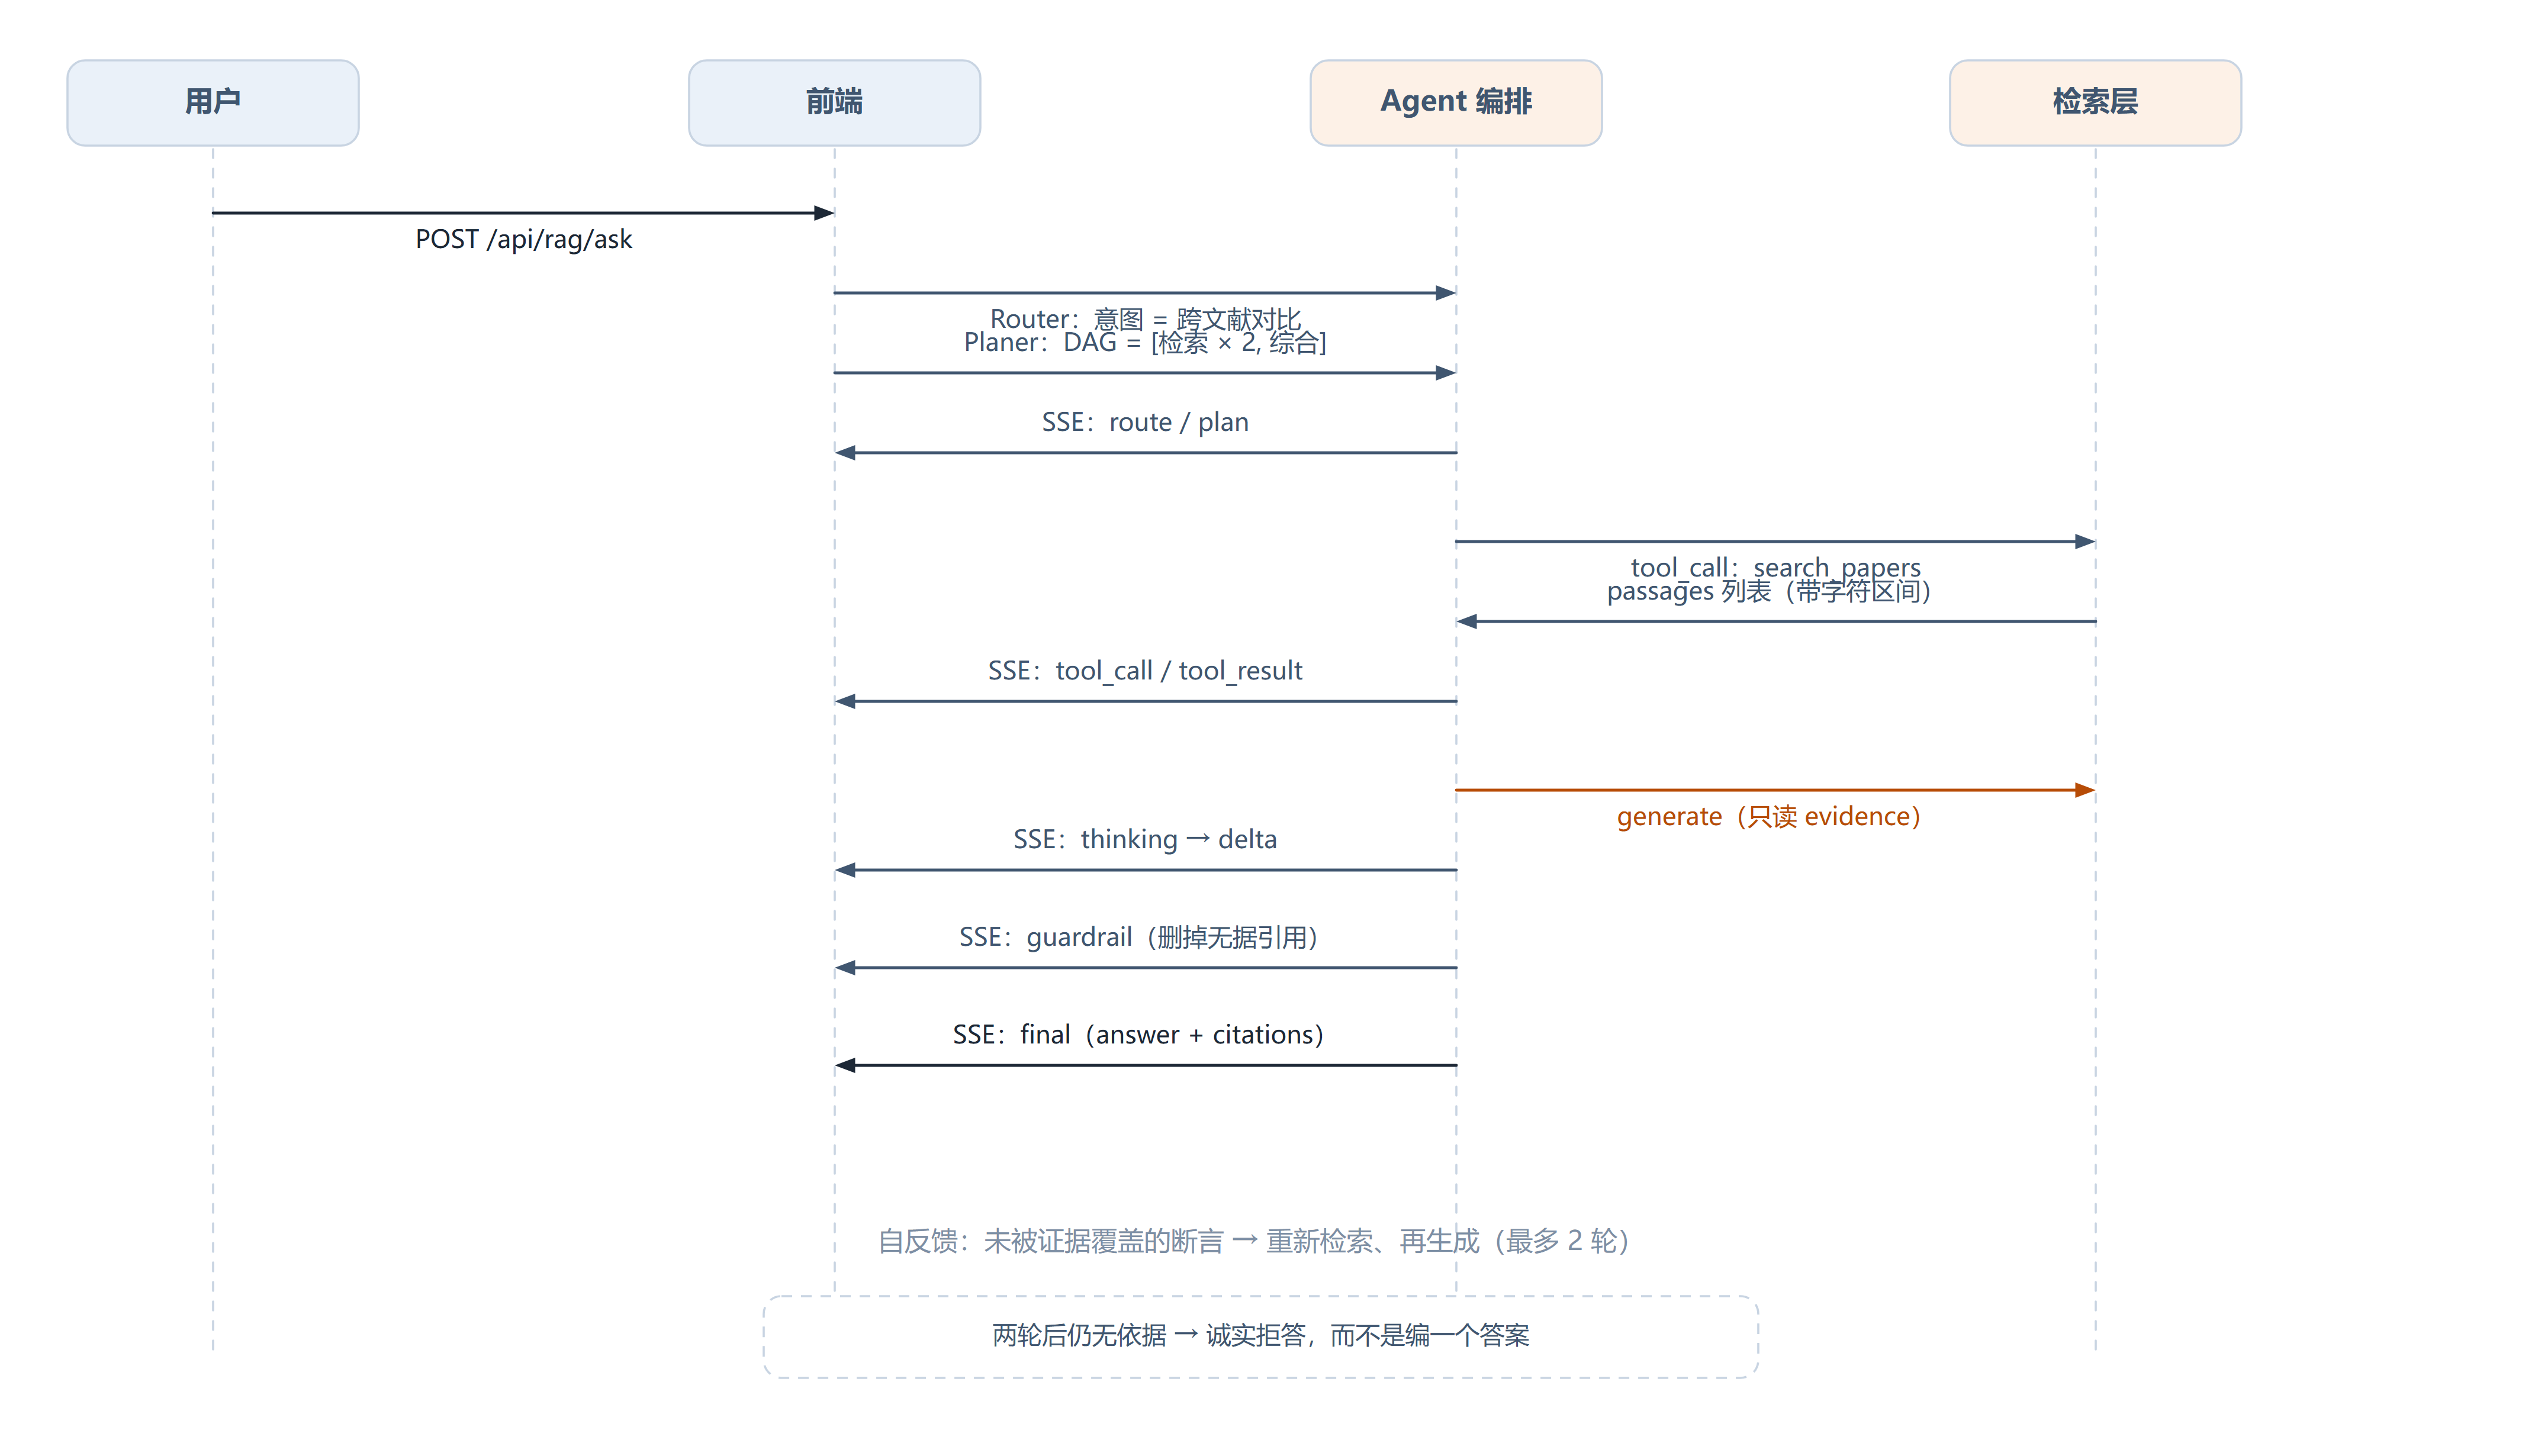
\includegraphics[width=0.88\textwidth]{figures/fig-seq.png}
\caption{一次跨文献问答的时序。SSE 事件逐条回推至前端，末条为带引用的答案}
\end{figure}

事件流共十二类，分别为 \texttt{session}、\texttt{route}、\texttt{plan}、\texttt{stage}、\texttt{thinking}、\texttt{tool\_call}、\texttt{tool\_result}、\texttt{delta}、\texttt{guardrail}、\texttt{final}、\texttt{error} 与 \texttt{abstain}。前端以统一的 \texttt{AgentEvent} 类型分发，各面板按事件类型更新。

\subsubsection*{3.5 存储与索引设计}
元数据采用 SQLite 存储。选择 SQLite 而非关系型数据库服务的原因有三：其一，演示环境为单机；其二，无需运维；其三，异步驱动不会阻塞事件流。表结构覆盖全部解析产物，包括论文、章节、分块、参考文献、图、表、公式与推荐反馈。

向量索引采用每篇论文一个矩阵文件的布局，而非单一的全局矩阵。其依据是内存占用：一次查询通常只涉及一至三篇文献，以内存映射方式仅将这几篇的分块向量载入地址空间，索引内存因而与库规模解耦。在 39 篇论文、1024 维、每篇约 3000 个分块的规模下，查询期的向量常驻内存为数百 KB，而非数十 MB。

分块依章节边界切分，块内按句子聚合，目标长度 380 token，重叠 60 token。章节边界保证语义完整，重叠则避免答案恰落在切点之上。

\subsubsection*{3.6 部署架构}
演示环境采用单进程同源托管，如图 3-4 所示。

\begin{figure}[htbp]
\centering
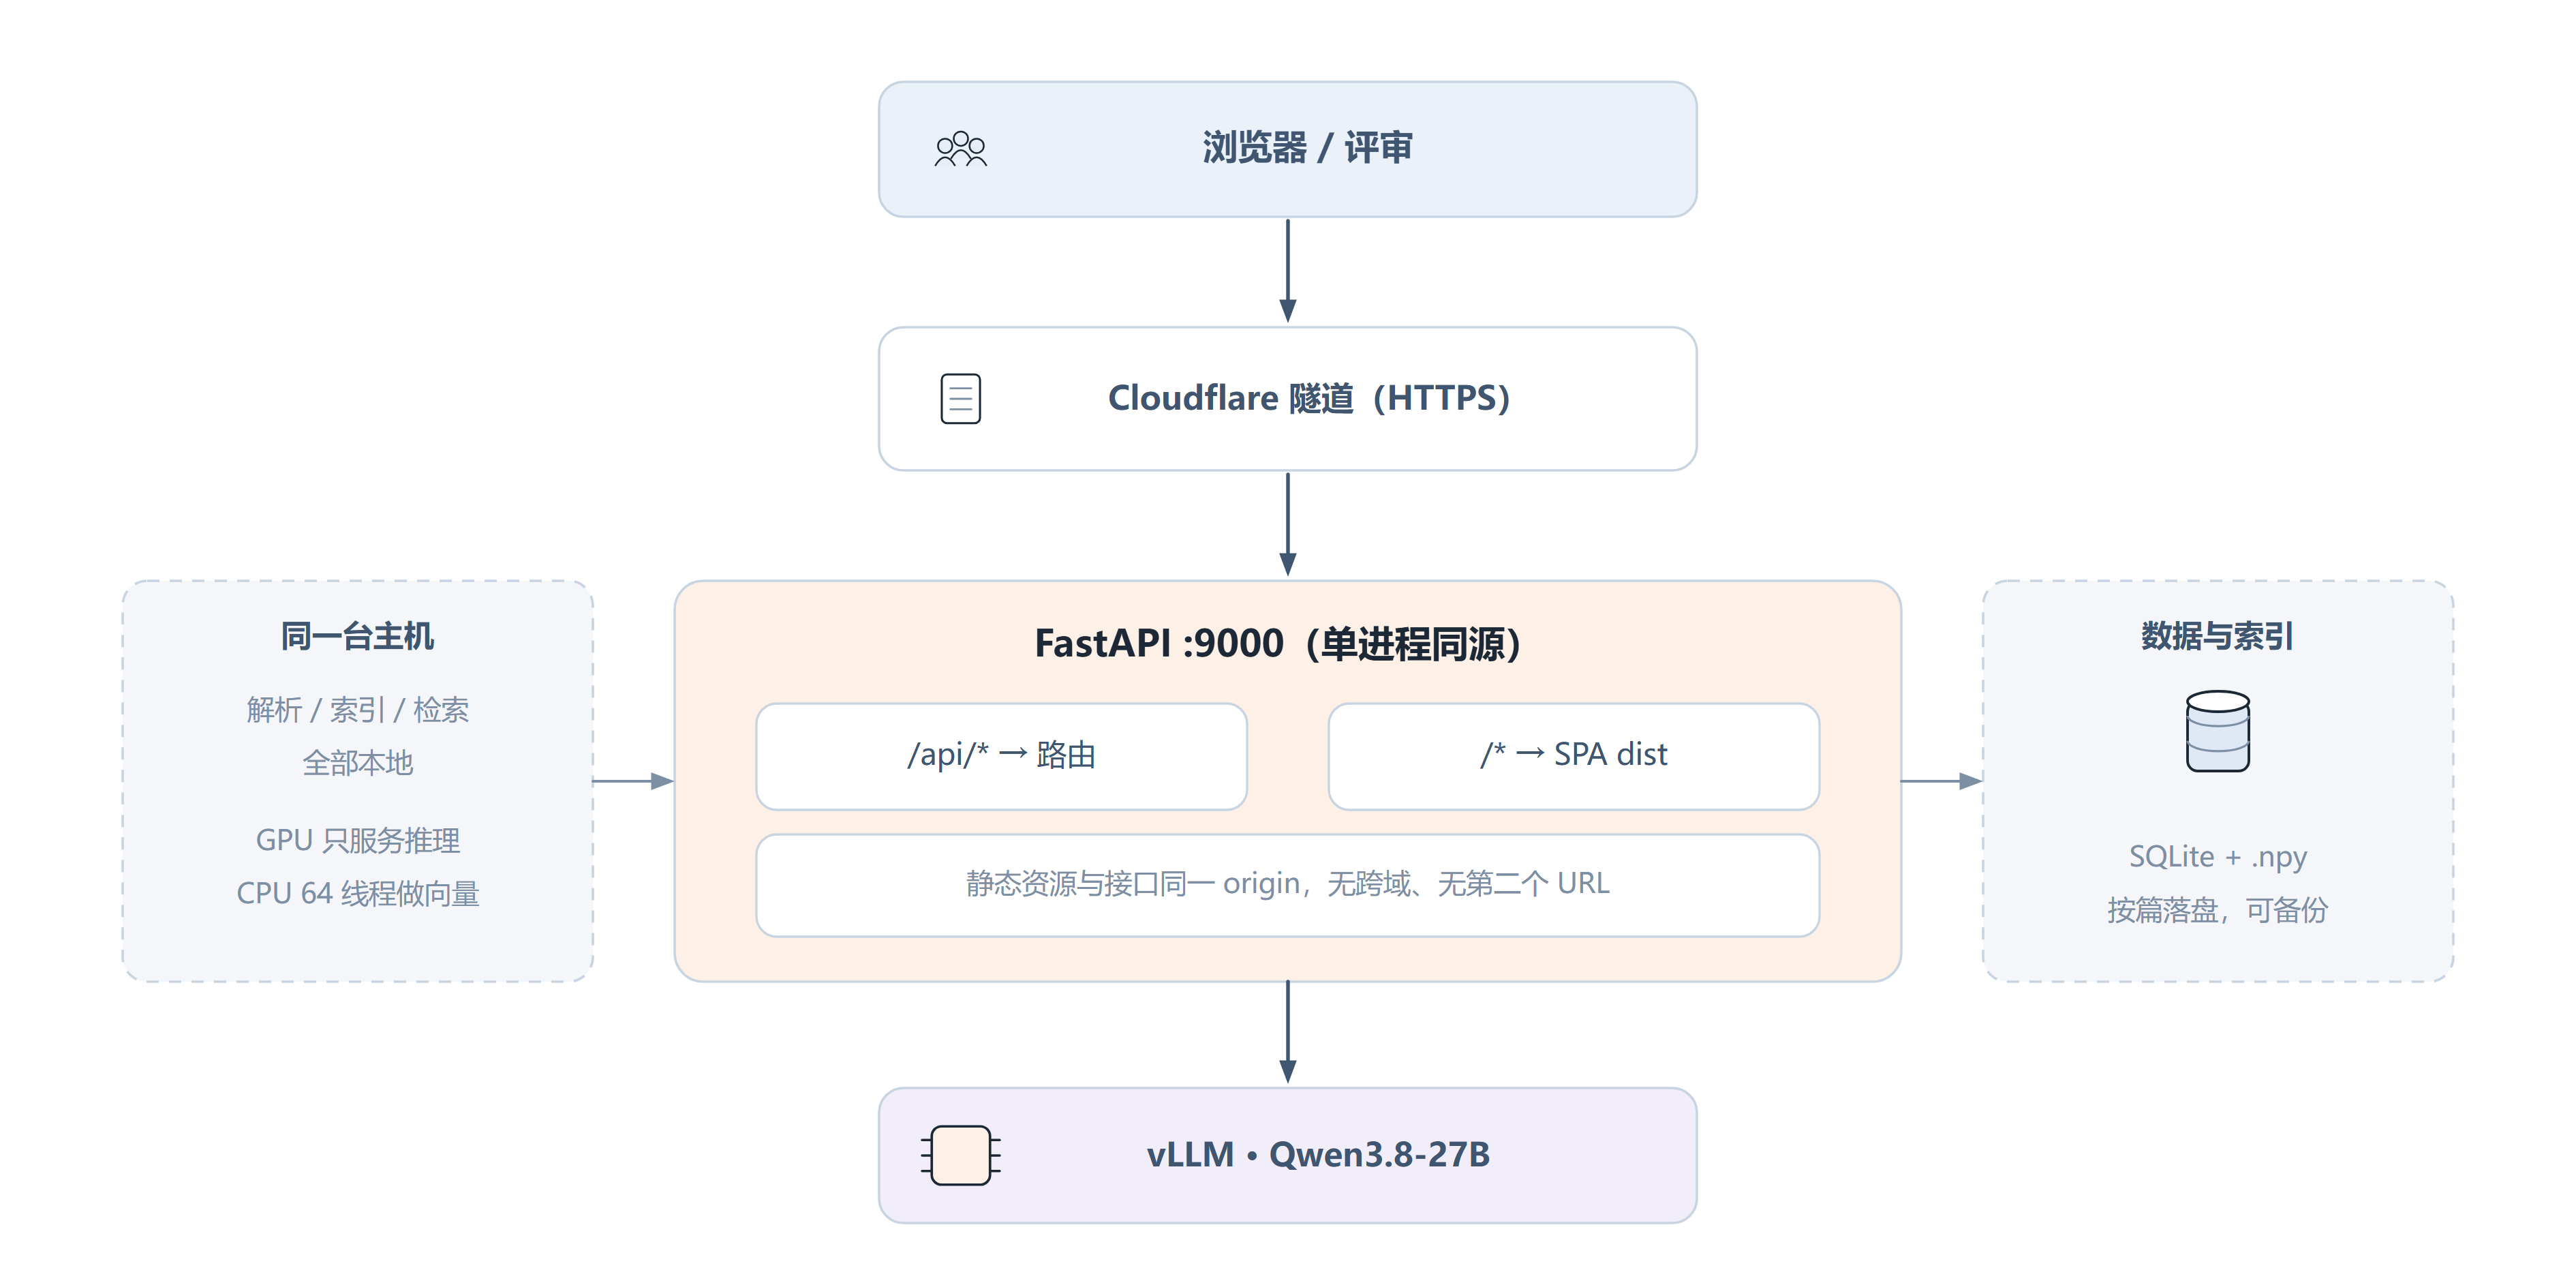
\includegraphics[width=0.88\textwidth]{figures/fig-deploy.png}
\caption{单进程同源的部署链路。隧道仅暴露一个 HTTPS 入口，接口与静态资源同源}
\end{figure}

部署形态在实施过程中收敛为单进程。初版方案将前端容器、后端容器与反向代理部署于一台独立的容器主机；实施中该主机失联，表现为双向 ping 100\% 丢包与 SSH 连接超时，而承载模型推理与密集计算的 192 核主机不具备容器权限，原拓扑无法落地。

收敛为单进程同源托管后，进程数、反向代理层与跨域配置各减少一层，部署与排障成本相应降低，接口与代码保持不变。仓库中仍保留三服务的容器编排文件，供具备容器权限的机器复现，详见 §6.6。

\begin{aside}运行时要求接口与前端资源处于同一源。前端以环境变量构造请求前缀，默认值为 \texttt{/api}，该前缀不可拆分；反向代理与单进程托管均满足此条件，差别仅在部署方式。\end{aside}

\subsection*{4. AI 技术方案}
\addcontentsline{toc}{subsection}{4. AI 技术方案}
本章按选型理由、集成方式与优化策略三部分展开，依次对应 §4.1 至 §4.2、§4.3 至 §4.7、§4.8 至 §4.10。

\subsubsection*{4.1 大模型选型与理由}
\textbf{选定方案：以 vLLM 自托管 Qwen3.8-27B，经 OpenAI 兼容协议接入。}

选型理由按重要性排序如下。

\begin{longtable}{@{}p{0.249\textwidth}p{0.711\textwidth}@{}}
\toprule
\multicolumn{1}{c}{\textbf{理由}} & \multicolumn{1}{c}{\textbf{具体依据}} \\
\midrule
\endfirsthead
\toprule
\multicolumn{1}{c}{\textbf{理由}} & \multicolumn{1}{c}{\textbf{具体依据}} \\
\midrule
\endhead
\bottomrule
\endfoot
\textbf{必须支持多模态} & 扫描件 OCR 与公式转写依赖读图能力。实测该模型架构为 \texttt{Qwen3\_5ForConditionalGeneration}，属多模态 VLM，传入 PNG 可准确读出图内标题与正文结构。 \\
须支持原生工具调用 & 工具循环依赖模型输出结构化的 \texttt{tool\_calls}；实测以 \texttt{--enable-auto-tool-choice} 启动后，模型可稳定返回该数组，参数符合 JSON Schema 约定。 \\
\textbf{必须提供 reasoning 字段} & Agent 思考过程的可视化是评分点之一。vLLM 对该模型返回独立的 \texttt{reasoning} 字段，可直接透传至前端 \texttt{thinking} 事件，无需从正文中推测。 \\
\textbf{私有化部署，零 API 成本、零外网依赖} & 比赛与评审期间不能依赖商用 API 的配额与稳定性，自托管 vLLM 可保证离线可复现。 \\
\textbf{上下文足够长} & \texttt{max\_model\_len = 262144}，多篇文献的证据可一次性放入生成阶段，无需多轮拼接。 \\
\textbf{可替换性} & 客户端只依赖 OpenAI 兼容协议，任何兼容端点均可通过 \texttt{LLM\_BASE\_URL} 接入，OpenAI、DeepSeek 与 Qwen API 均属此列，前提是模型具备多模态与 function calling 能力。 \\
\end{longtable}

关于模型规模，本人取 27B，使其在自托管成本与能力之间取得平衡。该规模的可行性来自系统结构：结构化解析、精确检索与图论计算均由确定性代码承担，模型只负责语义理解与自然语言生成，输出因而更为稳定。

\subsubsection*{4.2 集成方式}
协议层统一采用 OpenAI 兼容的 \texttt{/v1/chat/completions}。\texttt{app/llm/client.py} 封装三项能力：

\begin{itemize}
\item \texttt{complete(...)}：普通对话，流式返回 token；
\item \texttt{complete\_json(...)}：结构化输出，依次为 schema hint 提示、JSON 解析与失败重试；
\item \texttt{stream\_with\_tools(...)}：带 \texttt{tools} 定义的工具循环，返回 \texttt{delta} / \texttt{reasoning} / \texttt{tool\_calls} 三类增量。
\end{itemize}

工具层由 \texttt{app/tools/registry.py} 以 \texttt{@tool} 装饰器完成注册，每个工具声明 JSON Schema、处理器与审计用途标签。Executor 把可用工具的 schema 转为 OpenAI 的 \texttt{tools} 参数；模型返回 \texttt{tool\_calls} 后，由注册表分发执行，结果以 \texttt{role: tool} 消息回灌，直至模型不再请求工具或达到 \texttt{AGENT\_MAX\_STEPS}。

已注册的工具依次为 \texttt{search\_papers}、\texttt{get\_paper\_structure}、\texttt{get\_references}、\texttt{arxiv\_search}、\texttt{arxiv\_download}、\texttt{check\_reproducibility}、\texttt{build\_citation\_graph}、\texttt{generate\_framework} 与 \texttt{plot\_csv}，分别承担本地混合检索、标题树获取、参考文献获取、arXiv 检索、arXiv 下载、GitHub 可复现性检查、引用图构建、框架生成与 CSV 绘图。

流式层：后端以 FastAPI 的 \texttt{StreamingResponse} 产出 \texttt{text/event-stream}；前端以 \texttt{fetch} 与 \texttt{ReadableStream} 逐块解析，未采用 \texttt{EventSource}，原因是该链路需要携带 POST body。请求须经 Nginx 转发，因此 \texttt{proxy\_buffering off} 是 SSE 生效的硬性前提，该配置在 \texttt{deploy/nginx.conf} 中有详细注释。

\subsubsection*{4.3 Prompt 工程}
系统提示词分五组，每组针对一个阶段，实现位于 \texttt{app/llm/prompts.py}。

\begin{longtable}{@{}p{0.317\textwidth}p{0.145\textwidth}p{0.498\textwidth}@{}}
\toprule
\multicolumn{1}{c}{\textbf{组}} & \multicolumn{1}{c}{\textbf{作用}} & \multicolumn{1}{c}{\textbf{关键设计}} \\
\midrule
\endfirsthead
\toprule
\multicolumn{1}{c}{\textbf{组}} & \multicolumn{1}{c}{\textbf{作用}} & \multicolumn{1}{c}{\textbf{关键设计}} \\
\midrule
\endhead
\bottomrule
\endfoot
\texttt{SYSTEM\_ROUTER} & 意图分类 & 要求输出受限的意图标签与所需工具集合，使路由结果可预测 \\
\texttt{SYSTEM\_PLANNER} & 任务拆解 & 要求输出 JSON 形式的子任务 DAG，每项含 \texttt{goal} / \texttt{tool} / \texttt{depends\_on} \\
\texttt{SYSTEM\_ANSWER} & 带证据生成 & \textbf{显式列出可用编号}，并规定只允许引用这些编号；要求证据不足时明确说明 \\
\texttt{SYSTEM\_REVIEW} & 综述生成 & 注入图指标与基石文献摘要，要求区分基石与衍生并给出依据 \\
\texttt{SYSTEM\_FRAMEWORK} / \texttt{SYSTEM\_DIAGRAM} & 写作辅助 & 框架生成要求参考文献只能取自给定的真实清单；架构图要求输出可编译的源码 \\
\end{longtable}

Prompt 设计遵循三条原则。

\begin{enumerate}
\item 约束可验证。所有 prompt 的输出均可由代码检查：字段是否齐全由 \texttt{complete\_json} 经 \texttt{validate\_structure} 校验，引用编号是否落在证据集内由 \texttt{bind\_citations} 校验，参考文献是否真实存在由 \texttt{validate\_references} 校验。"请不要编造"只是一句劝告，"编号超出范围会被删除"则构成可执行的约束。
\item 注入防护。检索到的文档正文经 \texttt{sanitize\_document\_text} 处理，疑似指令的片段被包裹进 \texttt{[untrusted-content]...[/untrusted-content]} 标记，使指令与数据在提示词层面分离。
\item 审慎输出。JSON 解析失败后重试一次；仍未成功则降级为纯文本并记录审计，不向用户抛出异常。
\end{enumerate}

\subsubsection*{4.4 Guardrails：六层学术安全防护}
\begin{longtable}{@{}p{0.185\textwidth}p{0.319\textwidth}p{0.456\textwidth}@{}}
\toprule
\multicolumn{1}{c}{\textbf{防护}} & \multicolumn{1}{c}{\textbf{实现}} & \multicolumn{1}{c}{\textbf{触发时的表现}} \\
\midrule
\endfirsthead
\toprule
\multicolumn{1}{c}{\textbf{防护}} & \multicolumn{1}{c}{\textbf{实现}} & \multicolumn{1}{c}{\textbf{触发时的表现}} \\
\midrule
\endhead
\bottomrule
\endfoot
\textbf{证据绑定} & \texttt{bind\_citations} & 删除无据引用标记，答案标记为 \texttt{supported: false}，UI 显示"已移除 N 个无据引用" \\
\textbf{引用真实性校验} & \texttt{validate\_references} & 幻觉引用进入"已拦截"列表，不进入最终参考文献 \\
\textbf{提示注入隔离} & \texttt{sanitize\_document\_text} & 文档中的指令被标记为不可信内容，模型不予执行 \\
结构化输出校验 & \texttt{validate\_structure} 与 \texttt{complete\_json} & 缺字段时自动重试一次，仍未成功则降级 \\
\textbf{无据拒答} & \texttt{requires\_abstention} & 返回明确说明与三条可操作建议，不给猜测性答案 \\
空答案按生成失败处理 & \texttt{\_generate\_answer} 与 \texttt{\_reflect} & 空的生成结果被判为\textbf{生成失败}，不再视为没有断言的正确答案：触发自反馈重试并将预算翻倍、发出 \texttt{generation\_failed} 事件、护栏判为不通过；重试后仍为空则\textbf{诚实拒答}，不返回空字符串 \\
\end{longtable}

这六层彼此独立。即便第 1 层漏掉一个引用编号，第 2 层仍会检查参考文献真实性；即便模型绕过前四层，第 5 层的空证据检查仍会触发；即便模型给出了正文，第 6 层还会检查该正文是否确实生成。由此构成纵深防御。

第 6 层为后续补充，起因是一次真实缺陷：跨论文题曾返回空答案，却因没有断言而被前五层全部放行，最终显示为护栏通过。该缺陷的完整取证与修复见 §4.10。一条没有内容的答案比一条有内容的错误答案更需警惕，因为它表面上呈现为系统未检索到，实质上可能是系统未生成。

\subsubsection*{4.5 混合检索：策略与理由}
\begin{figure}[htbp]
\centering
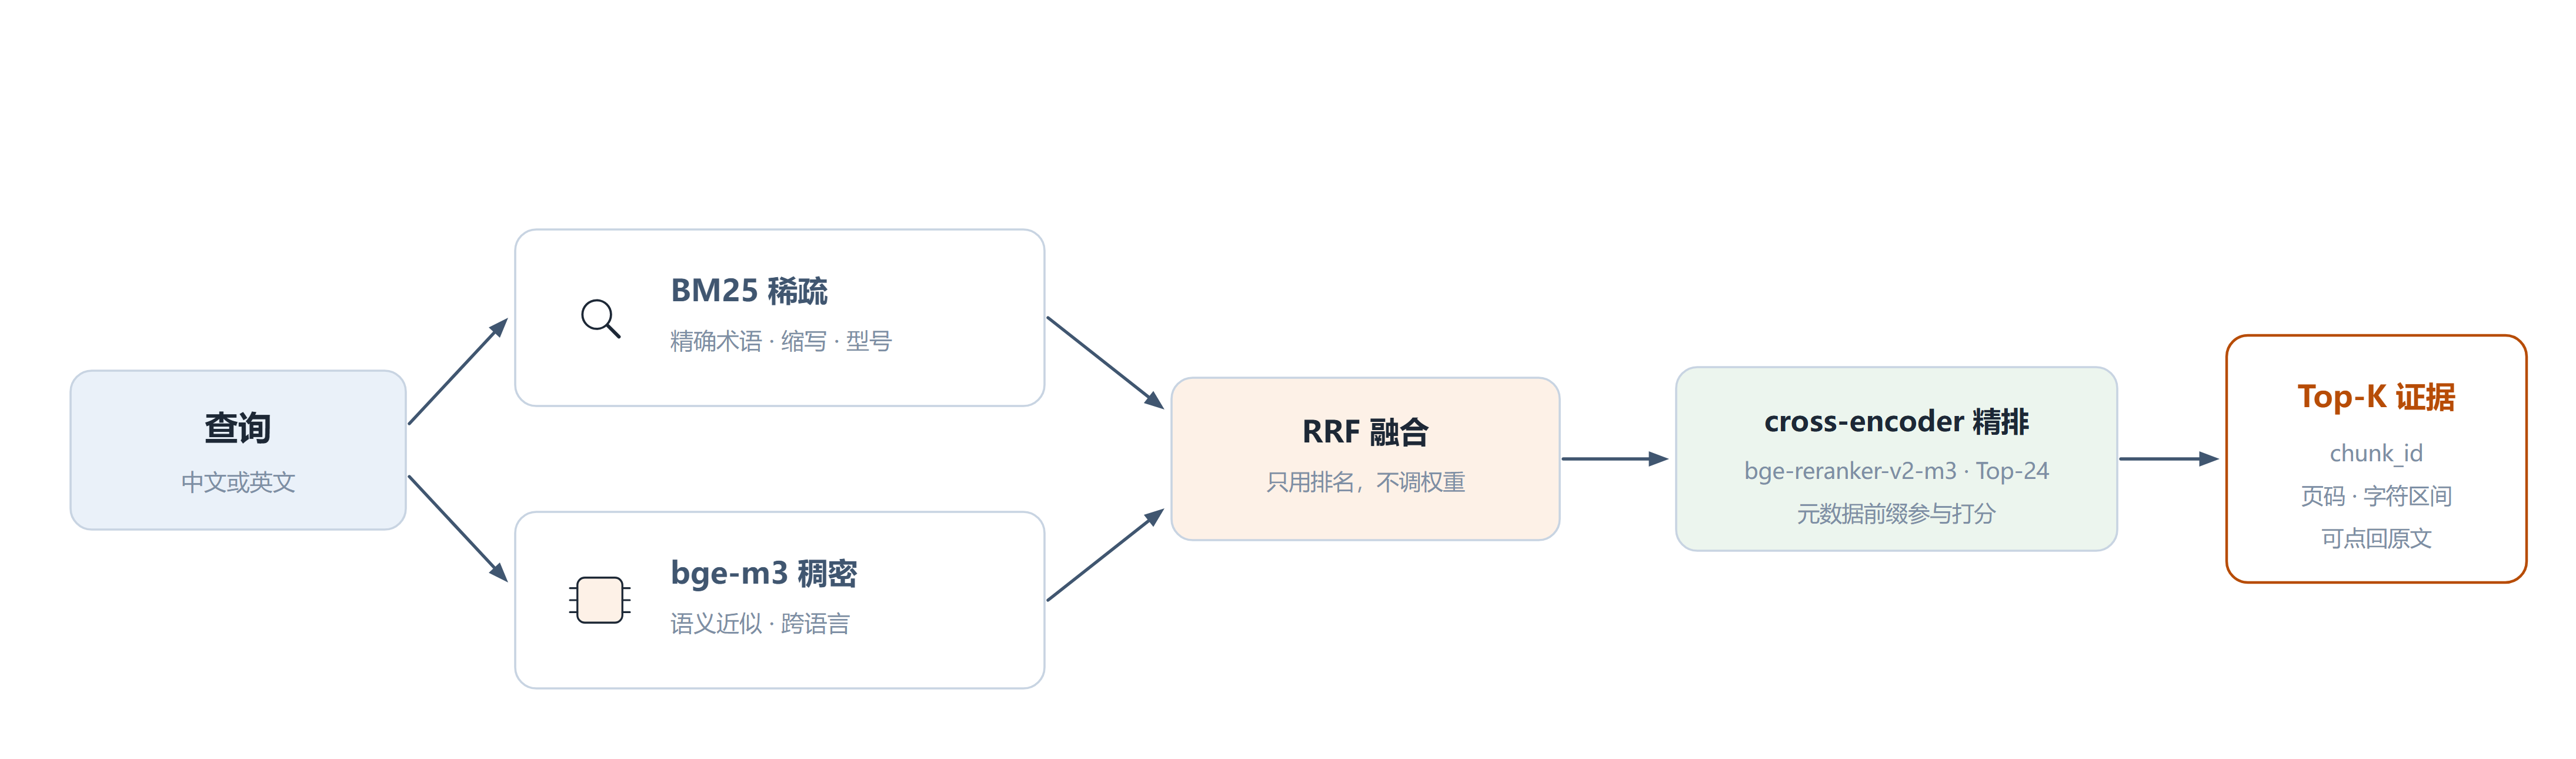
\includegraphics[width=0.88\textwidth]{figures/fig-retrieval.png}
\caption{混合检索链路。两路召回各自打分，只用排名融合，再交给精排}
\end{figure}

检索采用两路召回。

\begin{itemize}
\item BM25 擅长精确术语、缩写与数字，例如 \texttt{multi-head attention}、\texttt{BLEU}、\texttt{P100}。这类词在科研提问中出现频率高且必须精确命中，纯稠密检索容易将其模糊化。
\item bge-m3 擅长语义近似与跨语言，原生支持中英混合与 8192 token 长文本，满足双语检索的需要。
\item 两路覆盖的查询类型不同，故采用 RRF 融合。
\end{itemize}

融合采用 RRF。BM25 分数无界，可达数十；余弦相似度有界，取值 0–1。加权求和须先归一化，而归一化方式本身引入调参与不稳定。RRF 仅使用排名，其形式为 \texttt{score(d) = Σ\_r 1/(k + rank\_r(d))}，无需归一化与调参，Elasticsearch 与 Azure AI Search 亦采用该做法。

重排作为召回后的第二级。双塔模型分别编码查询与段落，二者之间没有交互；cross-encoder 将 (query, passage) 拼接后做联合注意力，可捕捉细粒度匹配。在本文的查询上，重排把正确段落由第 2 位提升至第 1 位，离题段落的打分由 +0.92 降至 +0.00。

两路通道与重排器的实测打分由脚本 \texttt{scripts/probe\_models.py} 测得，结果如下。

\begin{Verbatim}[fontsize=\scriptsize,breaklines=true,breakanywhere=true,frame=single,framerule=0.2pt,rulecolor=\color{rule}]
dense : sim(相关) = 0.8895    sim(无关) = 0.3784
rerank: 切题段落 +0.9234 / +0.9441     离题段落 +0.0000
\end{Verbatim}

\subsubsection*{4.6 图论算法选型}
在引用有向图上同时计算四类指标，各有分工。

\begin{longtable}{@{}p{0.310\textwidth}p{0.240\textwidth}p{0.410\textwidth}@{}}
\toprule
\multicolumn{1}{c}{\textbf{算法}} & \multicolumn{1}{c}{\textbf{判别目标}} & \multicolumn{1}{c}{\textbf{在本文中的作用}} \\
\midrule
\endfirsthead
\toprule
\multicolumn{1}{c}{\textbf{算法}} & \multicolumn{1}{c}{\textbf{判别目标}} & \multicolumn{1}{c}{\textbf{在本文中的作用}} \\
\midrule
\endhead
\bottomrule
\endfoot
\textbf{PageRank} & 影响力最大的文献 & 基石判定的主指标，取随机游走视角 \\
\textbf{Betweenness Centrality} & 承担桥接作用的文献 & 识别承上启下的枢纽文献，去除该节点即割裂知识流 \\
\textbf{k-core} & 核心团的凝聚程度 & 度量核心团的厚度，k-core 高的节点属于紧密协作的核心 \\
\textbf{HITS} 枢纽与权威度量 & 引用权威或连接枢纽的文献 & 补充 PageRank 对入度与出度不对称性的刻画 \\
\end{longtable}

基石判定不采用单一的 PageRank。单用 PageRank 会把被引多与被不同群体引混为一谈：一篇被 50 篇同组论文引用的综述，PageRank 很高但桥接作用弱；一篇被 5 个不同子领域引用的方法论文，PageRank 不高但 betweenness 很高。因此本人以多指标联合判定作为基石的界定方式。

基石判定规则位于 \texttt{app/graph/builder.py}，综合入度、PageRank 排名、k-core 与年份，划分 \texttt{foundation} / \texttt{core} / \texttt{derivative} 三档。年份参与判定，用以排除近两年新出且被大量引用所造成的引用膨胀效应。

引用质量分析由 \texttt{filter\_substantive\_references} 完成，区分实质性引用与装饰性引用。判据包括引用所在句子是否与被引文献的标题共享词汇、是否附着于定量或比较性论断，例如 \texttt{outperform}、\texttt{state-of-the-art} 与含数字的表述，以及是否仅为一句"see [12]"。该分析使用户得以判断某篇论文的实质学术依托。

\subsubsection*{4.7 多模态解析与 OCR}
版式解析由 \texttt{app/parsing/layout.py} 实现：以 PyMuPDF 的词级 bbox 为基础做栏聚类，将页面按 x 间隙切分为 1 列或 2 列，再按左栏读完继续右栏的顺序输出。这一步决定了双栏论文的正文是否可读，是整个系统的基础。

标题树推断由 \texttt{app/parsing/headings.py} 实现，联合三条证据判定：（1）显式编号模式，\texttt{3.2.2} 归入 level 3；（2）规范章节名，如 \texttt{Introduction}、\texttt{Related Work} 与 \texttt{Conclusion}；（3）排版特征，包括字号大于正文 8\%、加粗与独占一行。同时设有一组负向规则专门排除误判，涉及论文左侧竖排的 arXiv 戳记，其形如 \texttt{arXiv:1706.03762v1 [cs.CL] 12 Jun 2017}，以及形如 \texttt{Figure 3:} 的图注、参考文献条目与正文段落。

VLM OCR 由 \texttt{app/parsing/ocr.py} 实现：页面文本层字符数低于阈值即判定为扫描件，逐页以 150 DPI 栅格化为 PNG，送入多模态模型转写并输出 Markdown。采用 VLM 的理由是 tesseract 在双栏顺序与数学公式上表现很差，它只看到字符，不理解版面，而多模态模型可同时读出结构、公式与栏序。转写结果再经 \texttt{ocr\_markdown\_to\_sections} 还原为标题树，因此扫描件论文同样具备可检索的章节结构。

并发上以 \texttt{asyncio.Semaphore} 限流，默认 4 路，使 15 页的转写耗时由串行的 >15 分钟压缩到约 4 分钟，同时避免超出 vLLM 的并发窗口。

语义去重由 \texttt{app/parsing/dedup.py} 实现，以四路证据联合判定同一论文：文件 SHA-256、规范化正文哈希、arXiv id 与 SimHash 近似度，并叠加标题 Jaccard 与摘要 embedding 余弦。命中后给出保留建议，比较 arXiv 版本号，版本号缺失时以正文长度兜底，并可输出逐行差异。

\subsubsection*{4.8 优化策略}
本节记录实测得出的优化项，每项均有数字支撑。

\subsubsection*{（1）线程池规模：13.8× 的吞吐差距}
在 192 核的机器上，torch 默认按核心数开启 192 个线程。对 bge-m3 这类中等规模模型，线程数远超有效并行度后，同步开销抵消了并行收益：

\begin{longtable}{@{}p{0.544\textwidth}p{0.416\textwidth}@{}}
\toprule
\multicolumn{1}{c}{\textbf{配置}} & \multicolumn{1}{c}{\textbf{吞吐，单位为 passages/s}} \\
\midrule
\endfirsthead
\toprule
\multicolumn{1}{c}{\textbf{配置}} & \multicolumn{1}{c}{\textbf{吞吐，单位为 passages/s}} \\
\midrule
\endhead
\bottomrule
\endfoot
\texttt{torch.get\_num\_threads() = 192}，默认值 & \textbf{7.2} \\
显式设为 32 线程 & 76.0 \\
\textbf{显式设为 64 线程} & \textbf{99.7} \\
192 线程，\texttt{max\_seq\_length} 取 256 & 99.5 \\
\end{longtable}

结论：显式限制线程数是必要的优化。实现见 \texttt{app/rag/embeddings.py::\_configure\_threads}，由 \texttt{EMBEDDING\_THREADS} 控制，默认 64。对应到完整索引 3000 个分块，耗时由 7 分钟降至 30 秒。

\subsubsection*{（2）GPU 不可用时的正确降级}
实测 8 张 L40 均被 vLLM 占用，GPU0 剩余 0.8 GB，bge-m3 加载时出现 OOM。因此稠密通道默认走 CPU，配置项为 \texttt{EMBEDDING\_DEVICE=cpu}，显存允许时可直接改为 \texttt{cuda}。该做法较默认 GPU、失败再降级的方案更为稳妥，降级路径不宜承担主路径的可靠性责任。

\subsubsection*{（3）模型权重获取：并发分块下载}
实验室内 HF 镜像在 2.2 GB 权重上会\textbf{卡死在 0 B/s}，实测 20 秒内零字节增长。改用 ModelScope 的 \texttt{resolve} 端点后，文件被切成 16 MB 分块、以 24 路并发拉取，2.27 GB 权重\textbf{约 4 分钟}完成。\texttt{scripts/download\_models.py} 实现了该下载器，含分块、校验、断点跳过与失败重试，并作为仓库脚本提供，评审可直接复现。

\subsubsection*{（4）分块粒度}
本人将目标定为 380 token，重叠 60 token。分块过大则单块语义稀释、rerank 精度下降；分块过小则上下文断裂、答案需要跨块拼接。380 是实测下检索精度与答案完整性之间的平衡点。

\subsubsection*{（5）按需加载向量}
采用 \texttt{.npy} 与 \texttt{mmap\_mode="r"}，查询期只把参与检索的论文分块映射进内存。39 篇论文的完整索引常驻内存为几百 KB 量级，库规模扩大时内存增长线性且可控。

\subsubsection*{（6）两阶段架构带来的流式优化}
工具调用与正文生成分为两阶段后，前端可在证据阶段即渲染正在检索哪些文献的思考面板，正文生成阶段则为纯粹的 token 流。用户感知的首屏延迟由等待模型完成思考变为立即看到进度。

\subsubsection*{（7）并发解析：将 CPU 密集段移出事件循环}
第一版实现把逐页的文本块提取、图表与公式抽取以及页面渲染直接写在 \texttt{async def} 函数体内。这在功能上正确，但存在一个隐蔽而致命的问题：这些同步的 CPU 密集调用会独占事件循环。后果有三：

\begin{enumerate}
\item SSE 进度通道被饿死，解析期间事件无法发出，前端进度条停滞；
\item 批量上传退化为串行，FastAPI 的 \texttt{BackgroundTasks} 本身串行执行，叠加事件循环阻塞后，第二篇文档必须等第一篇彻底结束；
\item 评分标准明确要求的多文档并发分析无法实现。
\end{enumerate}

修复分两步。

第一步，把 CPU 密集段下沉到线程池。PyMuPDF 的文本抽取与页面渲染在执行期间释放 GIL，因此按页并行是真正并行的：

\begin{Verbatim}[fontsize=\scriptsize,breaklines=true,breakanywhere=true,frame=single,framerule=0.2pt,rulecolor=\color{rule}]
# app/parsing/pipeline.py
loop = asyncio.get_running_loop()
extracted = await asyncio.gather(
    *(loop.run_in_executor(None, _extract_one, i) for i in indices)
)
\end{Verbatim}

第二步，把批量上传改为受信号量保护的并发任务。弃用 \texttt{BackgroundTasks}，因其串行执行，改为向事件循环派发任务并以信号量限流：

\begin{Verbatim}[fontsize=\scriptsize,breaklines=true,breakanywhere=true,frame=single,framerule=0.2pt,rulecolor=\color{rule}]
# app/api/routers/papers.py
_PARSE_CONCURRENCY = 3
...
asyncio.create_task(_ingest_guarded(path, filename, paper_id, allow_duplicate))
\end{Verbatim}

并发度取 3 而未取更高值：解析消耗的是 CPU 带宽，OCR 消耗的是 vLLM 的并发窗口，两者瓶颈不同；且 8 张 L40 已被大模型服务占满，留出余量转发 OCR 更为稳妥。

附带收益：上传即创建 \texttt{status="parsing"} 的占位行，解析期间文献库即可看到该条目及其状态；解析失败时把错误写回该行并置为 \texttt{failed}，条目不会无故消失。

\subsubsection*{（8）并发解析}
页面级解析由 \texttt{PARSE\_WORKERS} 控制进程池并行，默认 8；OCR 以信号量限流到 4 路。前者消耗 CPU 带宽，后者消耗 vLLM 的并发窗口，两者瓶颈不同，因此分开调参。

\subsection*{4.9 缺陷复盘之一：外键约束与工作单元插入顺序}
\addcontentsline{toc}{subsection}{4.9 缺陷复盘之一：外键约束与工作单元插入顺序}
本节记录开发过程中定位并修复的一处缺陷。该缺陷源于对 ORM 语义的误解，而非业务逻辑错误，其成因与排查过程具有一定代表性。

现象为文献库始终为空。解析、识别与索引三项均成功，但持久化函数落库时抛出如下异常：

\begin{Verbatim}[fontsize=\scriptsize,breaklines=true,breakanywhere=true,frame=single,framerule=0.2pt,rulecolor=\color{rule}]
sqlite3.IntegrityError: FOREIGN KEY constraint failed
[SQL: INSERT INTO content_blocks (id, paper_id, section_id, page_no, ...)]
[parameters: [('34578353...', '517f55ad...', None, 1, 'text', ...), ... 479 rows]]
\end{Verbatim}

排查过程分两步。先将问题缩减为最小复现：仅创建一行论文记录与五行内容块记录，不建立其余表，异常依然出现，据此排除数据、并发与事务提交三类原因。随后开启语句回显，取得决定性证据：内容块表的插入语句先于论文记录执行，随即回滚。

根因在于工作单元的排序依据。SQLAlchemy 的工作单元依 ORM 关系图推导插入顺序，而不依据表级外键约束。本系统中内容块、表格、图与公式四张子表仅声明了指向论文表的外键，未声明对应的关系属性，ORM 因而无从得知其依赖于论文表，将这四张表视为彼此独立参与排序。内容块表恰为本次事务中字典序最靠前者，其插入遂被排在论文记录之前，父行尚不存在，外键检查随即拒绝整批写入。

修复分两层。模型层为四张子表补充反向关系声明，使 ORM 的依赖图真实反映表的父子关系，此为根治之处。服务层在持久化函数中先落盘父行，再挂载子行，将顺序约束由隐式的 ORM 排序改为显式的两段写入。

诊断脚本保留了五个对照变体，分别为裸外键、父行先行落盘、仅含关系声明的模型、赋值关系对象与完整修复路径。修复后五个变体全部通过；其中裸外键变体亦能通过，说明模型层的补齐方为根本原因所在。

该缺陷属于建表成功而写入失败的一类。开发期间单表查询、解析逻辑与前端展示均正常，仅端到端写入路径失败；此类缺陷不会在单元测试中暴露，因为测试通常只验证解析结果而不验证落库。为此，本人补充了一条以真实写入路径为断言的回归测试，见 §6.2。

\subsection*{4.10 缺陷复盘之二：推理通道耗尽令牌预算导致空答案被判为合格}
\addcontentsline{toc}{subsection}{4.10 缺陷复盘之二：推理通道耗尽令牌预算导致空答案被判为合格}
较之前一节，该缺陷更为隐蔽：无异常、无报错，界面显示正常，护栏亦报告通过。

现象为赛题点名的四道跨论文题中有两道返回空答案，而引用条目为 26 至 33 条，说明证据检索正常；护栏报告为支持，不支撑比例为 0.0，自反馈轮次为 0。检索与证据均无问题，护栏亦判为通过，唯独答案为空。

初次定位时，本人的直觉是零断言即零不支撑，因而准备修改护栏。动手之前先核查该次调用本身。系统在审计表中保留每次模型调用的完整轨迹，查询结果如下：

\begin{Verbatim}[fontsize=\scriptsize,breaklines=true,breakanywhere=true,frame=single,framerule=0.2pt,rulecolor=\color{rule}]
purpose=agent:answer  ok=1  prompt_tok=9508  completion_tok=4096
latency_ms=213786  resp_len=0  reason_len=8000
\end{Verbatim}

四个字段即可还原全过程：补全令牌数恰等于上限 4096，响应长度为 0，即正文未写出任何字符，而推理长度为 8000，即推理通道写满预算；调用状态记为成功，因为结束原因为长度而非错误。

成因分三层，各层单独看均属合理，叠加之后形成静默失败。

\begin{longtable}{@{}p{0.138\textwidth}p{0.497\textwidth}p{0.325\textwidth}@{}}
\toprule
\multicolumn{1}{c}{\textbf{层}} & \multicolumn{1}{c}{\textbf{行为}} & \multicolumn{1}{c}{\textbf{后果}} \\
\midrule
\endfirsthead
\toprule
\multicolumn{1}{c}{\textbf{层}} & \multicolumn{1}{c}{\textbf{行为}} & \multicolumn{1}{c}{\textbf{后果}} \\
\midrule
\endhead
\bottomrule
\endfoot
模型 & 推理通道与正文共享同一令牌预算。跨论文题的提示达 9508 令牌，推理耗尽预算，正文未写出任何字符 & 结束原因为长度，客户端视为正常返回 \\
客户端 & 流式调用遇异常时产出一帧错误事件 & 编排器仅处理推理、增量与完成三类事件，错误帧被丢弃 \\
编排器 & 答案为空导致覆盖度报告返回空值，自反馈循环随即退出 & 自反馈未被触发 \\
护栏 & 空答案中不存在引用标签，待删除集合为空，判定为支持 & 空答案通过校验 \\
\end{longtable}

修复分四层，每层均有对应的回归用例：

\begin{enumerate}
\item 不丢弃错误。错误帧被记录为生成错误并作为失败原因上报，不再静默处理。
\item 空答案视为失败。答案为空即判定生成失败，进入自反馈循环，以问题本身作为补检索查询重写，并将令牌预算加倍。
\item 护栏不误判。空答案的支持标志必须为假，并在说明中标注生成结果为空、无可校验断言。
\item 诚实拒答。自反馈之后答案仍为空，则返回拒答，而非空字符串。
\end{enumerate}

根本性的修复在于避免预算被推理通道占用。Qwen3 的对话模板提供推理开关，本文将其配置化，分为 Agent 阶段与答案阶段两项。Agent 阶段的推理决定工具序列的合理性，且会流式呈现为界面的思考面板，故予以保留；答案阶段的证据已在提示之中，故默认关闭。同一道题的实测结果如下。

\begin{longtable}{@{}p{0.166\textwidth}p{0.260\textwidth}p{0.235\textwidth}p{0.146\textwidth}p{0.153\textwidth}@{}}
\toprule
\multicolumn{1}{c}{\textbf{答案阶段}} & \multicolumn{1}{c}{\textbf{耗时}} & \multicolumn{1}{c}{\textbf{补全令牌}} & \multicolumn{1}{c}{\textbf{正文}} & \multicolumn{1}{c}{\textbf{推理}} \\
\midrule
\endfirsthead
\toprule
\multicolumn{1}{c}{\textbf{答案阶段}} & \multicolumn{1}{c}{\textbf{耗时}} & \multicolumn{1}{c}{\textbf{补全令牌}} & \multicolumn{1}{c}{\textbf{正文}} & \multicolumn{1}{c}{\textbf{推理}} \\
\midrule
\endhead
\bottomrule
\endfoot
开启推理 & 简单题 4.2 秒；跨论文题 214 秒且无答案 & 166；跨论文题 4096，触及上限 & 有；跨论文题为空 & 385 字符；写满 \\
关闭推理 & 0.8 秒 & 34 & 有 & 0 \\
\end{longtable}

修复后重跑此前完全空白的那道跨论文题，系统给出了完整的承袭与抛弃对照表，每个单元格附引用标签，标签依次为 [16] [15] [18] [1] [20] [12] [4] [23] [17]，并给出带引用的结论段。

该缺陷的价值在于其表现形态：系统并未崩溃，而是看起来一切正常。既无异常堆栈，也无告警，护栏甚至报告通过。若验收流程仅检查接口返回码与护栏结论，此次失败将被判为成功。定位该缺陷所依据的并非运行日志，而是调用审计记录；这也说明审计轨迹本身即是重要的可观测性来源。

\subsection*{5. 核心功能实现}
\addcontentsline{toc}{subsection}{5. 核心功能实现}
\subsubsection*{5.1 模块一：多模态与细粒度文档解析}
实现要点如下。

\begin{itemize}
\item \texttt{app/parsing/layout.py}：先做词级 bbox 提取，再作栏聚类，最终按栏序输出；合并行成段，并保留 \texttt{page\_no} 与 \texttt{bbox}。
\item \texttt{app/parsing/headings.py}：依据编号、规范名与排版三类证据判定标题，并以负向规则排除 arXiv 戳记、图注与参考文献。
\item \texttt{app/parsing/metadata.py}：标题取首页首个居中大字号块；作者依 \texttt{∗} 标记符识别，并以机构名排除；同时抽取机构、摘要、arXiv id、版本号与会议信息，会议信息仅扫描首页，以避免误匹配参考文献中的会议名。
\item \texttt{app/parsing/references.py}：将参考文献条目解析为作者、标题、年份、venue、DOI 与 arXiv id，并回链库内论文。
\item \texttt{app/parsing/extractors.py}：表格经 PyMuPDF 的 \texttt{find\_tables()} 输出 Markdown 与 CSV；图片按提取结果与就近 caption 处理；公式按行内与块级两种模式处理。
\item \texttt{app/parsing/ocr.py}：先检测扫描件，再作栅格化，随后由 VLM 转写，最后还原章节。
\item \texttt{app/parsing/dedup.py}：按四路指纹去重，给出推荐版本，并输出逐行 diff。
\end{itemize}

本文以 \texttt{1706.03762v1.pdf} 作为实测样本，该文为 Attention Is All You Need，全文 15 页，结果如下表。

\begin{longtable}{@{}p{0.294\textwidth}p{0.666\textwidth}@{}}
\toprule
\multicolumn{1}{c}{\textbf{项}} & \multicolumn{1}{c}{\textbf{结果}} \\
\midrule
\endfirsthead
\toprule
\multicolumn{1}{c}{\textbf{项}} & \multicolumn{1}{c}{\textbf{结果}} \\
\midrule
\endhead
\bottomrule
\endfoot
版式解析耗时，不含公式 LaTeX 转写 & \textbf{4.2 秒} \\
端到端耗时，含 27 条公式的 VLM 转写 & 71.7 秒 \\
标题 & \texttt{Attention Is All You Need} ✓ \\
作者 & \textbf{8 位全部正确}，含第 6 位 \texttt{Aidan N. Gomez}，其机构为 University of Toronto，直接对应赛题第 1 问 \\
机构 & 3 条 ✓ \\
摘要 & 1566 字符 ✓ \\
arXiv ID / 版本 & \texttt{1706.03762} / \texttt{v1} ✓ \\
标题树 & \textbf{26 个章节节点}，最深 3 级，正确包含 \texttt{3.2.2 Multi-Head Attention} ✓ \\
表 / 图 / 公式 & 4 / 7 / 27 ✓ \\
参考文献 & \textbf{71 条结构化}，例：\texttt{Jimmy Lei Ba, Jamie Ryan Kiros, and Geoffrey E Hinton. Layer normalization...} ✓ \\
\end{longtable}

同一论文的 v7 版 \texttt{1706.03762v7.pdf} 测得 4.4 秒、26 节、75 条参考文献、4 表、7 图、27 公式，为版本去重与版本差异对比提供了真实样本。

\begin{aside}两项耗时口径须予区分。4.2 秒对应版式与结构抽取，由 \texttt{parse\_smoke.py} 以 \texttt{transcribe\_formulas=False} 测得；完整入库还需将 27 条公式的裁剪图交多模态模型转写为 LaTeX，端到端耗时为 71.7 秒。前者衡量解析器自身的工程质量，后者反映入库环节的实际延迟，两者不宜混同。\end{aside}

本轮工作中，本人的改动重点落在公式的版式还原上。

在 LaTeX 生成的 PDF 中，大号运算符 \texttt{∑} 的字形包围盒与同行基线错位，PyMuPDF 因而把一条显示公式切分为多个 block；上下标同时被当作独立 span 读出。界面上呈现的即为 \texttt{i log P(ui|ui−k, ...)} 一类失去层次的字串。相关修改集中在 \texttt{parsing/layout.py} 中。

\begin{longtable}{@{}p{0.342\textwidth}p{0.618\textwidth}@{}}
\toprule
\multicolumn{1}{c}{\textbf{机制}} & \multicolumn{1}{c}{\textbf{作用}} \\
\midrule
\endfirsthead
\toprule
\multicolumn{1}{c}{\textbf{机制}} & \multicolumn{1}{c}{\textbf{作用}} \\
\midrule
\endhead
\bottomrule
\endfoot
\texttt{\_visual\_rows()} & 将切碎的同一"印刷行"合回一行，判据为垂直重叠 ≥ 50\% 且水平间距 ≤ 6pt \\
\texttt{\_attach\_limits()} & 将 CMEX 字体大运算符下方的极限移回运算符所在行，并把 CMEX 的 \texttt{X} 还原为 \texttt{∑} \\
\texttt{\_row\_texts()} & 按几何关系还原上下标，得到 \texttt{W\_\{e\}}、\texttt{x\textasciicircum{}\{1\}}、\texttt{u\_\{i−k\}}、\texttt{h\textasciicircum{}\{m\}\_\{l\}}；句中用作引文标注的上标数字不作公式处理 \\
\texttt{\_merge\_equation\_fragments()} & 依据数学字体、行重叠与水平重叠三重判据，跨 block 合并同一条显示公式 \\
\end{longtable}

改前与改后的对比如下，样本为 BERT 论文第 3 页，相关截图已核对。

\begin{Verbatim}[fontsize=\scriptsize,breaklines=true,breakanywhere=true,frame=single,framerule=0.2pt,rulecolor=\color{rule}]
改前：  L₁(U) = ∑                              ← 独立一块
        i log P(u_i|u_{i−k}, …, u_{i−1}; Θ) (1)  ← 独立一块

改后：  L_{1}(U) = ∑_{i} log P(u_{i}|u_{i−k}, …, u_{i−1}; Θ)(1)   ← 一块
\end{Verbatim}

公式以页面裁剪图呈现，与表格一致；裁剪范围取合并后的 block bbox，整条式子因而落在图内。LaTeX 作为折叠的补充信息，由 VLM 直接读取裁剪图转写，合并之后转写质量同步提升，得到 \texttt{\textbackslash\{\}sum\_\{i\}\textbackslash\{\}log P(u\_\{i\}|u\_\{i-k\},\textbackslash\{\}ldots,u\_\{i-1\};\textbackslash\{\}Theta)}。公式块不进入正文，也不参与翻译，但保留在 \texttt{full\_text} 中供检索。回归用例见 T44–T46。

\subsubsection*{5.2 模块二：抗幻觉 RAG 与 Agent 编排}
见 §4.3–§4.5。实现文件及其职责如下：\texttt{app/rag/retriever.py} 承担混合检索，\texttt{app/rag/chunker.py} 承担分块，\texttt{app/rag/sparse.py} 承担 BM25 与 RRF，\texttt{app/rag/embeddings.py} 承担稠密检索与重排，\texttt{app/rag/meta\_aware.py} 承担元数据亲和度，\texttt{app/rag/evaluation.py} 承担三个指标，\texttt{app/agents/orchestrator.py} 承担编排，\texttt{app/llm/guardrails.py} 承担护栏。

溯源锚点方面，每个分块均携带 \texttt{paper\_id}、\texttt{page\_no}、\texttt{char\_start} 与 \texttt{char\_end}，答案中每一个引用编号都可反查上述字段，前端点击后即跳转至阅读器的对应页面。

生成之后另有两个步骤，共同构成第三阶段。

\begin{enumerate}
\item 按断言级完成引用对齐修复。模型经常把标签指错，例如作者名单位于 \texttt{[3]}，答案却写作 \texttt{[9]}。系统以规则定位每条断言，找出真正支持该断言的证据块，再改写标签；同时把该条引文替换为真正支持这句断言的那一段原文，段落开头的 320 字符不足以承担这一作用。界面上呈现的引文与指标核算所用的引文为同一段文字。
\item 自反馈推理循环。答案生成后，以 §6.3 的规则化指标检查每条断言是否由其自身引用所支持，此处不采用 LLM 评审。若存在证据缺口，则以未被支持的断言构造新的检索式，再检索一轮并重新撰写答案，最多两轮。缺口判断之所以不交由 LLM 完成，是因为 Agent Laboratory 的实测显示，LLM 评审对自身给出的分数为 6.1/10，远高于人类专家的 3.8/10，该文见 arXiv:2501.04227。
\end{enumerate}

生成预算方面，答案阶段另设独立的 token 预算，由 \texttt{llm\_answer\_max\_tokens} 控制，并默认关闭模型的推理通道，对应配置项 \texttt{llm\_answer\_thinking=false}。证据已置于 prompt 之中，模型无须再把预算用于思考，实测收益见 §4.10 的对照表，其中耗时为 0.8 s 与 4.2 s，token 消耗为 34 tokens 与 166 tokens。空答案的处理一并从严：空答案一律计为生成失败，不被当作缺少断言的正确答案。此情形会触发自反馈重试并将预算翻倍，同时发出 \texttt{generation\_failed} 事件，护栏亦判为不通过；若重试后答案仍为空，系统返回明确拒答，而不返回空字符串。整条链路设有四个回归用例，编号为 T35–T38。

\subsubsection*{5.3 模块三：版式阅读器与中英双向联动}
界面采用三栏布局。左侧为标题树，层级可展开，点击即跳转至对应页面；中间为原文页面图，保真渲染并不作重排，学术阅读需要保留原始版式；右侧为中英对照。

中英联动依托对齐后的 segment 列表实现。翻译先产出完整的 \texttt{\{index, source, translation, kind, page\_no\}} 结构，左右两栏渲染同一份列表，滚动时按比例同步位置。据此段落始终一一对应，不会出现左栏第 3 段与右栏第 5 段相配的错位。

引用支持双向跳转。正文中的 \texttt{[11]} 可点击并打开对应的参考文献条目；条目上列出引用该文献的句子，并可据此反向跳转回正文。

\subsubsection*{5.4 模块四：arXiv 检索、追踪与可复现性}
\begin{itemize}
\item \texttt{arxiv\_search}：直连 arXiv API，支持关键词检索。
\item \texttt{arxiv\_recent}：按分类拉取最新提交，用于定期追踪。
\item \texttt{arxiv\_download}：下载 PDF 后自动解析入库，并返回该文献是否重复。
\item \texttt{github\_repos}：经 GitHub Search API 查找论文对应的公开仓库。
\item 推荐排序：\texttt{score = 0.6 × 内容相关度 + 0.25 × (有公开代码) + ≤0.15 × 用户反馈}。
\end{itemize}

将可复现性设为权重 0.25 的独立硬信号，未按微调因子处理，原因是赛题明确要求优先推荐可复现的工作。相关度以文献库标题与摘要构成的领域画像同候选标题、摘要之间的词汇重叠度计算，无须额外的模型调用。

\subsubsection*{5.5 模块五：引用图谱与基石挖掘}
见 §4.6。实现文件包括 \texttt{app/graph/builder.py}，负责图构建与指标计算；\texttt{app/graph/future\_work.py}，负责机会挖掘；\texttt{app/api/routers/graph.py}，负责接口。

Future Work 机会挖掘的流程如下。分块阶段即通过 \texttt{FUTURE\_WORK\_TITLES} 标记标题含 "Future Work"、"Limitations"、"Discussion" 或 "Open Problems" 的章节；挖掘器先收集这些片段，再作去重，随后交由大模型归纳为研究机会，每个机会附有新颖性论证、难度、影响力与来源论文。所生成的机会须具备可执行性，仅替换原句表述的做法不予采用。

\subsubsection*{5.6 模块六：论文写作助手}
框架生成环节设有防幻觉设计。\texttt{generate\_framework} 工具先从库内检索真实参考文献并交予模型，模型仅可从这份清单中选取；结果返回后再执行 \texttt{validate\_references} 作二次校验，未通过的条目移入 \texttt{rejected\_references}，界面中单独列为护栏拦截的幻觉引用。

架构图支持 Mermaid、TikZ 与 Graphviz 三种形式，任选其一。Mermaid 经 \texttt{mermaid.render} 在前端实时渲染，并支持下载 SVG；TikZ 与 DOT 以源码形式提供，可直接复制到论文中。

图表与 Caption 的生成由 \texttt{app/tools/viz.py} 完成。该模块先解析 CSV，再由 matplotlib 渲染出版级图形，图形类别可选；随后由大模型生成 Figure Caption 与关键结论，并同时输出 Markdown 数据表。图形、caption 与数据表在一次调用中一并产出，该环节在论文写作中机械性与耗时程度均较高。

\subsubsection*{5.7 前端：六个工作台}
\begin{longtable}{@{}p{0.158\textwidth}p{0.226\textwidth}p{0.575\textwidth}@{}}
\toprule
\multicolumn{1}{c}{\textbf{页面}} & \multicolumn{1}{c}{\textbf{路由}} & \multicolumn{1}{c}{\textbf{要点}} \\
\midrule
\endfirsthead
\toprule
\multicolumn{1}{c}{\textbf{页面}} & \multicolumn{1}{c}{\textbf{路由}} & \multicolumn{1}{c}{\textbf{要点}} \\
\midrule
\endhead
\bottomrule
\endfoot
文献库 & \texttt{/library} & 批量上传并显示 XHR 进度、实时解析状态、勾选后供下游模块使用 \\
阅读器 & \texttt{/reader/:id} & 三栏布局、引用双向跳转、中英联动 \\
智能问答 & \texttt{/ask} & 思考过程面板、token 级流式输出、引用卡片、护栏报告 \\
图谱综述 & \texttt{/graph} & Cytoscape 渲染，节点颜色表示角色、节点大小表示 PageRank；指标表、自动综述、Future Work 与引用质量 \\
检索推荐 & \texttt{/search} & arXiv 检索、智能推荐与最新追踪，下载入库，支持点赞与点踩反馈 \\
写作工作台 & \texttt{/writing} & 框架生成、架构图与图表及 Caption，架构图支持 Mermaid 实时预览 \\
\end{longtable}

设计系统基于 Tailwind 自定义 token。\texttt{ink} 为深蓝灰，用于主操作；\texttt{parchment} 为暖白，用于阅读面；\texttt{accent} 为琥珀色，用于 Agent 正在思考的状态；\texttt{teal} 用于引用与代码标识。衬线体用于论文正文与标题，以保持学术观感；无衬线体用于界面；JetBrains Mono 用于代码与指标数字。深色模式得到完整支持。

\#\# 6. 测试与部署

\subsubsection*{6.1 测试策略}
\begin{longtable}{@{}p{0.170\textwidth}p{0.556\textwidth}p{0.234\textwidth}@{}}
\toprule
\multicolumn{1}{c}{\textbf{层次}} & \multicolumn{1}{c}{\textbf{覆盖对象}} & \multicolumn{1}{c}{\textbf{是否依赖 LLM}} \\
\midrule
\endfirsthead
\toprule
\multicolumn{1}{c}{\textbf{层次}} & \multicolumn{1}{c}{\textbf{覆盖对象}} & \multicolumn{1}{c}{\textbf{是否依赖 LLM}} \\
\midrule
\endhead
\bottomrule
\endfoot
单元测试 & 哈希、SimHash、BM25、RRF、分块、标题树、护栏、图指标、元数据抽取、评测指标、矛盾检测、引用修复 & 否 \\
集成测试 & 真实 PDF 解析、真实模型编码与重排 & 否，需本地权重 \\
端到端 & SSE 问答流、OCR、arXiv 下载 & 是 \\
\end{longtable}

\texttt{backend/tests/} 下共 \textbf{16 个测试文件、227 个用例}，全部可在无网络、无 LLM 的环境下运行；依赖真实 PDF 的用例在检测到本地文件时自动运行，否则标记为 \texttt{skip}。

另有以 \texttt{scripts/check\_undefined.py} 实现的静态作用域检查器，该检查器本身被固化为一条测试用例：它遍历 \texttt{backend/app} 的每个模块，借助 AST 找出“已读取但从未绑定、导入或作为参数传入”的名字，此类名字一旦存在，测试即失败。该检查的价值在 §8.1 的 T15 中说明。

\subsubsection*{6.2 测试用例与结果}
\begin{longtable}{@{}p{0.135\textwidth}p{0.244\textwidth}p{0.398\textwidth}p{0.183\textwidth}@{}}
\toprule
\multicolumn{1}{c}{\textbf{\#}} & \multicolumn{1}{c}{\textbf{用例}} & \multicolumn{1}{c}{\textbf{期望}} & \multicolumn{1}{c}{\textbf{实测}} \\
\midrule
\endfirsthead
\toprule
\multicolumn{1}{c}{\textbf{\#}} & \multicolumn{1}{c}{\textbf{用例}} & \multicolumn{1}{c}{\textbf{期望}} & \multicolumn{1}{c}{\textbf{实测}} \\
\midrule
\endhead
\bottomrule
\endfoot
T1 & 标准论文标题树 & 含 \texttt{3.2.2 Multi-Head Attention} & ✓ \\
T2 & 标准论文作者 & 8 位含 \texttt{Aidan N. Gomez} & ✓ \\
T3 & 标准论文参考文献 & ≥ 70 条且字段完整 & ✓ 76 条 \\
T4 & arXiv 戳记不误判为标题 & 无 \texttt{arXiv} 标题节点 & ✓ \\
T5 & 正文段落不误判为标题 & 无正文标题节点 & ✓ \\
T6 & 标题树嵌套 & \texttt{2.1.1} 的父节点为 \texttt{2.1} & ✓ \\
T7 & v1 与 v7 判定为同一论文 & \texttt{same\_paper = True} & ✓ \\
T8 & 版本推荐 & 保留 v7 & ✓ \\
T9 & 版本差异 & 输出行级 diff & ✓ \\
T10 & BM25 精确术语命中 & 命中含 \texttt{multi head attention} 的文档 & ✓ \\
T11 & RRF 双路融合 & 双路均靠前的文档排名更高 & ✓ \\
T12 & 分块可溯源 & 每个 chunk 均含 page 与 char range & ✓ \\
T13 & 稠密检索语义 & 相关 0.89 > 无关 0.38 & ✓ \\
T14 & 重排区分度 & 切题段落 0.92，离题段落 0.00 & ✓ \\
T15 & PageRank 归一 & 节点 PageRank 之和 = 1 & ✓ \\
T16 & 基石判定 & 被引最多的论文判为 foundation & ✓ \\
T17 & 引用质量分层 & 实质性引用与装饰性引用正确分离 & ✓ \\
T18 & 证据绑定 & 无据引用编号被删除 & ✓ \\
T19 & 幻觉引用拦截 & 不存在的文献进入 rejected & ✓ \\
T20 & 提示注入隔离 & 注入内容被标记 & ✓ \\
T21 & 无据拒答 & 空证据触发拒答 & ✓ \\
T22 & 结构化输出校验 & 缺字段被检出 & ✓ \\
T23 & 扫描件 OCR 与结构重建 & 标题、作者、摘要、标题树、参考文献均恢复 & ✓ \\
T24 & 541 页长文档 & 不 OOM、可解析 & ✓ 149.4 s、1254 章节、131 万字符 \\
T25 & 元数据年份推导 & \texttt{arXiv:1910.xxxxx} 不再落成 1910 & ✓ 1910 修正为 2019、2005 修正为 2020 \\
T26 & 摘要按栏提取 & 双栏论文的摘要不被清空 & ✓ Codex 摘要 2927 字 \\
T27 & TMLR 版式作者块 & 第 6 位作者与机构正确 & ✓ 《Emergent Abilities》由 0 增至 16 位作者 \\
T28 & 连字空格 & \texttt{Jeff Dean} 不粘连 & ✓ flags 198 \\
T29 & 静态作用域检查 & 无未绑定名字 & ✓ 0 告警，含自检用例 \\
T30 & 表格断言抽取 & 对比表格的单元格成为断言 & ✓ \\
T31 & 关键事实校验 & \texttt{eight A100 GPUs} 不被 \texttt{P100} 证据支持 & ✓ \\
T32 & 引用对齐修复 & 指向错误证据块的标签被纠正 & ✓ \\
T33 & 矛盾检测收紧 & 泛主语的结论冲突不误报 & ✓ 真实库误报由 3 降至 0 \\
T34 & 自反馈推理循环 & 证据缺口触发二次检索 & ✓ \\
T35 & 空答案不被接受 & 空答案触发自反馈重试，预算翻倍 & ✓ \\
T36 & 空答案护栏不报绿 & \texttt{supported=False} 与诚实拒答 & ✓ \\
T37 & LLM 失败帧不被吞 & \texttt{error} 帧触发 \texttt{generation\_failed} 事件 & ✓ \\
T38 & 答案阶段推理开关透传 & \texttt{thinking} 随配置下发 & ✓ \\
T39 & 对比断言按被引段落并集判定 & 跨论文对比句不再被误判为未支持 & ✓ \\
T40 & 分散断言需单段锚点 & 段落分散引用不能通过判定 & ✓ \\
T41 & 单段引用判定不变 & A100/P100 仍被拦下 & ✓ \\
T42 & 共有指标名不计为共有上下文 & “人类 95.6\% accuracy”与“模型 97\%-98\% accuracy on NSP”不判为矛盾 & ✓ 15 篇库误报由 2 条降至 0 \\
T43 & 排除指标名后真实冲突仍报出 & Attention 两版本 BLEU 41.0 与 41.8 仍被判为矛盾 & ✓ \\
T44 & 跨 block 合并显示公式 & 被 PyMuPDF 切碎的同一条公式合并为一条，裁剪图覆盖整式 & ✓ BERT p.3 由 2 块并为 1 块 \\
T45 & 行内上下标还原 & \texttt{W\_\{e\}} / \texttt{x\textasciicircum{}\{1\}} / \texttt{h\textasciicircum{}\{m\}\_\{l\}} 不再退化为 \texttt{We} / \texttt{x1} / \texttt{hm l} & ✓ \\
T46 & 两栏不误并公式 & 左右两栏各自的公式不被跨栏合并 & ✓ \\
\end{longtable}

自动化测试结果：\texttt{backend/tests/} 下 \textbf{16 个测试文件、227 个用例}，在无网络、无 LLM 的环境下可完整运行。容器内缺少真实 PDF 与 bge-m3 权重，结果为 \texttt{227 passed / 9 skipped}，耗时 2.4 秒；同一套用例在有 PDF 与权重的主机上为 \texttt{236 passed}，耗时 52 秒。依赖真实 PDF 的用例在检测到本地文件时自动运行，否则 \texttt{skip}；依赖本地权重的稠密与重排用例在检测到模型目录时自动运行。

\begin{aside}回归用例 1：测试套件中有一条断言要求表格被正确提取且数量 ≥ 3 张。该断言在表格提取移入线程池之后失败，说明其判定有效：该用例拦截了一个仅在端到端写入路径上暴露的缺陷，其表现为静默丢数据，即不报错而表格数量减少。详见 §4.9。\end{aside}

\begin{aside}回归用例 2：§6.3 的三个指标初测结果为 \texttt{0.00 / 0.67 / 0.25}。经逐条核对，该结果反映的是度量工具的缺陷：跨论文的两道对比题未产出任何断言，原因是答案为一张 Markdown 表格，而指标将表格整行丢弃；单论文题的忠实度偏低，原因是引文仅截取段落的前 320 个字符，而一个 chunk 的平均长度为 1274 个字符——\textbf{第 6 位作者位于第 1000 个字符处，事实已在证据之中，却被判为“未被支持”}。两处缺陷的修复过程见 §6.3。\end{aside}

\subsubsection*{6.3 三个 RAG 指标的实测}
\subsubsection*{6.3.1 指标不采用 LLM 评审的理由}
赛题关注的问题是“系统的回答是否忠于文献”。一种直观做法是引入大模型担任评审，但 Agent Laboratory 以 arXiv:2501.04227 提供了明确的反例：\textbf{LLM 评审对自身给出的评分为 6.1/10，远高于人类专家的 3.8/10}。会为自身打分的度量工具无法用于证明自身。因此本文的三个指标全部规则化，判定逻辑写在 \texttt{app/rag/evaluation.py}，每条规则均有对应的单元用例。

\begin{longtable}{@{}p{0.319\textwidth}p{0.385\textwidth}p{0.257\textwidth}@{}}
\toprule
\multicolumn{1}{c}{\textbf{指标}} & \multicolumn{1}{c}{\textbf{定义}} & \multicolumn{1}{c}{\textbf{解决的问题}} \\
\midrule
\endfirsthead
\toprule
\multicolumn{1}{c}{\textbf{指标}} & \multicolumn{1}{c}{\textbf{定义}} & \multicolumn{1}{c}{\textbf{解决的问题}} \\
\midrule
\endhead
\bottomrule
\endfoot
\texttt{faithfulness} & 答案的断言中，\textbf{被其自身所引用的那段原文支持}的比例 & 引用是否真正支持该句 \\
\texttt{citation\_traceability} & 引用编号中能\textbf{解析到已检索段落}的比例 & 读者能否点开溯源 \\
\texttt{context\_precision} & 已检索段落中\textbf{真正被答案使用}的比例 & 检索是否引入无关内容 \\
\end{longtable}

一条断言被判为“支持”，须同时满足三个条件：

\begin{enumerate}
\item \textbf{词项覆盖 ≥ 60\%}：断言的内容词在多大比例上出现于被引段落；
\item 关键事实全部对应：断言中的数字、型号与缩写，如 \texttt{41.0}、\texttt{A100}、\texttt{BLEU}、\texttt{WMT}，必须逐个出现在被引段落中；
\item 至少一段证据真正支撑该断言：被引段落中覆盖最好的一段单独达到 ≥ 30\%。
\end{enumerate}

第二个条件有其必要。纯词项覆盖会把“eight \textbf{A100} GPUs”判为被“eight \textbf{P100} GPUs”支持，覆盖率达 80\%，而答案写错了型号；关键事实校验正是拦截此类“形似”判定的环节。

第三个条件同样必要，作用方向则相反：一条断言引用多段证据时，按被引段落的并集判定。RAGAS 的口径是“断言是否被其引用的上下文支持”，判定对象为引用上下文整体；跨论文的对比句本就应由两篇论文各提供一半事实，任何单一段落都无法覆盖它。与此同时，必须有至少一段单独支撑该断言，否则“将全部段落一并挂上”即可通过判定。两条规则均有回归用例，见 T39、T40、T41。

\subsubsection*{6.3.2 首轮评测的 0.00 与度量工具缺陷的定位}
首轮评测共 9 题、13 篇库，得到 \texttt{faithfulness 0.204 / traceability 0.667 / precision 0.255}。该结果远低于预期，其性质更接近度量工具失效。逐条核对后，本人确认问题位于度量工具一侧，共四处缺陷，模型能力并未出现对应退化：

\begin{longtable}{@{}p{0.230\textwidth}p{0.441\textwidth}p{0.289\textwidth}@{}}
\toprule
\multicolumn{1}{c}{\textbf{现象}} & \multicolumn{1}{c}{\textbf{根因}} & \multicolumn{1}{c}{\textbf{修复}} \\
\midrule
\endfirsthead
\toprule
\multicolumn{1}{c}{\textbf{现象}} & \multicolumn{1}{c}{\textbf{根因}} & \multicolumn{1}{c}{\textbf{修复}} \\
\midrule
\endhead
\bottomrule
\endfoot
跨论文对比题\textbf{未产出任何断言} & 答案为一张 Markdown 表格，断言抽取将表格整行丢弃 & 表格单元格还原为“行标签、值、引用”构成的断言，值与原引用的绑定关系得以保留 \\
单论文题忠实度接近 0 & 引文仅截取段落\textbf{前 320 字符}，而 chunk 平均长度为 \textbf{1274 字符}；第 6 位作者位于第 1000 个字符处，\textbf{事实已在证据之中却被判为未支持} & 核验改为对\textbf{整段原文}进行；界面引文改为“真正支持该断言的那一句” \\
断言本身正确而忠实度仍低 & “who / listed / affiliated”一类\textbf{框架词}被计入分母，此类词属于句式框架，不构成断言内容 & 扩充学术语体停用词表，纳入框架词与通用学术动词 \\
“The paper notes that X”被整句判为未支持 & \textbf{归属前缀不属于断言内容}，原文中不会出现“the paper notes” & 增加归属前缀剥离规则 \\
\end{longtable}

上述四处修复均未调整系统以迎合指标，改动的对象均为度量工具。判断依据直接：若事实已出现在被引段落之中，指标仍判为“未被支持”，则指标判定有误。

\textbf{第二轮修复后为 0.685 / 0.778 / 0.328}，但按跨论文题拆分后又暴露出第五处度量工具缺陷：

\begin{longtable}{@{}p{0.082\textwidth}p{0.205\textwidth}p{0.318\textwidth}p{0.354\textwidth}@{}}
\toprule
\multicolumn{1}{c}{\textbf{\#}} & \multicolumn{1}{c}{\textbf{现象}} & \multicolumn{1}{c}{\textbf{根因}} & \multicolumn{1}{c}{\textbf{修复}} \\
\midrule
\endfirsthead
\toprule
\multicolumn{1}{c}{\textbf{\#}} & \multicolumn{1}{c}{\textbf{现象}} & \multicolumn{1}{c}{\textbf{根因}} & \multicolumn{1}{c}{\textbf{修复}} \\
\midrule
\endhead
\bottomrule
\endfoot
5 & 跨论文对比句虽具备证据，却大面积被判为未支持 & 判定采用 \texttt{max(单段覆盖率)}，而跨论文对比句本应由两篇论文各提供一半事实，任何单一段落都无法覆盖 & 依 RAGAS 口径改为\textbf{被引段落的并集}判定，并增设“至少一段单独覆盖 ≥ 30\%”的锚点，防止堆砌段落通过判定 \\
\end{longtable}

该处判据同样明确：RAGAS 的判定对象是断言与其所引用上下文整体的关系。并集判定必须配合锚点，否则答案只需将检索到的段落全部列出即可通过，故 T40 以一条“词项均匀分布于四段、无任何单段构成支撑”的断言封堵该路径。

本节所述的修复均针对判定规则；§4.10 所记的一次改动则指向真正的系统缺陷：跨论文题返回空答案而护栏显示通过。度量工具修复之后，空答案的评分仍为 0.00，可见度量与系统两侧须分别核查，否则易将度量失准误判为系统失效，或作相反归因。

五处度量工具缺陷与一处系统缺陷修复完成之后，同一套题连跑三轮，得到 \textbf{\texttt{faithfulness} 均值 0.7092，区间 0.6378 – 0.7521，\texttt{citation\_traceability} 三轮均为 1.0000}，对应 v4 / v5 / v6，即重建前的语料。此后语料因三处解析缺陷重建三次，分别为乱码修复、显示公式跨 block 合并与行内上下标还原；重建完成后以同一套题重跑三轮，得到 \textbf{\texttt{faithfulness} 均值 0.8034，\texttt{citation\_traceability} 三轮均为 1.0000}，对应 v10 / v11 / v12，即当前语料的冻结快照，详见 §6.3.4。此处不使用“单次最优成绩”的表述：三轮的离散度本身即为信息，仅报告较高一轮而隐去较低一轮有违严谨。

\subsubsection*{6.3.3 指标对“不支持”的判定：关键事实校验与对照问题}
指标不应只输出“支持”。为此设置两类反向检验：

\begin{itemize}
\item 单元层面：\texttt{eight NVIDIA A100 GPUs} 不被 \texttt{eight NVIDIA P100 GPUs} 支持；\texttt{It also won a Turing Award} 不被任何段落支持；\texttt{bleu 41.0} 不被 \texttt{bleu 41.8} 支持。
\item 系统层面：向系统提出三个库内无法回答的问题，即 CIFAR-10 验证损失、最佳论文奖与训练预算，观察其拒答还是编造。见 §6.3.5。
\end{itemize}

\subsubsection*{6.3.4 结果}
评测在 \textbf{15 篇真实库}上运行三轮，即 v10 / v11 / v12。题目取自赛题点名的两类场景：单篇论文的作者、超参、GPU、BLEU 与参考文献，以及跨论文的架构继承与参数增长对比。三轮运行于同一份冻结快照：语料在评测开始时复制为独立副本，由第二个独立后端实例提供服务，该实例使用独立端口与独立索引目录，演示实例不重启。由此，评测期间向演示库上传新论文不会改变评测语料。该做法系发现问题之后补充，见下文说明。

\begin{aside}\textbf{未采用 v4–v9 五次旧运行的原因}：v4 / v5 / v6 运行于重建前的语料，chunk 边界与检索命中均已改变，故作废；v7 / v8 / v9 则在评测过程中库发生变动——一篇 BERT 论文在第 1 轮与第 2 轮之间被上传，而 \texttt{papers.created\_at} 存储的是 UTC 时间，界面显示时间比实际入库时间早 8 小时，初期未被察觉。核对引用时该问题得以暴露：三轮各自引用该论文 \textbf{0 / 8 / 34} 次，同一道 BERT 题的忠实度分别为 \textbf{0.17 / 0.82 / 0.48}。三轮对应的库不同，数字不可平均，故整批作废并改用冻结快照重跑。\end{aside}

总体结果如下：

\begin{longtable}{@{}p{0.191\textwidth}p{0.115\textwidth}p{0.115\textwidth}p{0.115\textwidth}p{0.143\textwidth}p{0.180\textwidth}p{0.100\textwidth}@{}}
\toprule
\multicolumn{1}{c}{\textbf{指标}} & \multicolumn{1}{c}{\textbf{v10}} & \multicolumn{1}{c}{\textbf{v11}} & \multicolumn{1}{c}{\textbf{v12}} & \multicolumn{1}{c}{\textbf{均值}} & \multicolumn{1}{c}{\textbf{区间}} & \multicolumn{1}{c}{\textbf{标准差}} \\
\midrule
\endfirsthead
\toprule
\multicolumn{1}{c}{\textbf{指标}} & \multicolumn{1}{c}{\textbf{v10}} & \multicolumn{1}{c}{\textbf{v11}} & \multicolumn{1}{c}{\textbf{v12}} & \multicolumn{1}{c}{\textbf{均值}} & \multicolumn{1}{c}{\textbf{区间}} & \multicolumn{1}{c}{\textbf{标准差}} \\
\midrule
\endhead
\bottomrule
\endfoot
\texttt{faithfulness} & 0.7898 & 0.8168 & 0.8035 & \textbf{0.8034} & 0.7898 – 0.8168 & 0.0110 \\
\texttt{citation\_traceability} & 1.0000 & 1.0000 & 1.0000 & \textbf{1.0000} & 1.0000 – 1.0000 & 0 \\
\texttt{context\_precision} & 0.2874 & 0.2632 & 0.2867 & \textbf{0.2791} & 0.2632 – 0.2874 & 0.0112 \\
\end{longtable}

三轮共产生 \textbf{158 条断言}，其中 \textbf{104 条}被判为被引用证据支持；自反馈共触发 \textbf{28 轮}。三轮产物 \texttt{eval\_rag\_v10.json} / \texttt{v11} / \texttt{v12} 连同每条断言的完整引用清单一并入库，清单含 chunk\_id、论文、页码、章节与原句，文中每个数字均可离线复算。

分题结果如下，取三轮均值：

\begin{longtable}{@{}p{0.103\textwidth}p{0.330\textwidth}p{0.214\textwidth}p{0.200\textwidth}p{0.113\textwidth}@{}}
\toprule
\multicolumn{1}{c}{\textbf{类型}} & \multicolumn{1}{c}{\textbf{题目}} & \multicolumn{1}{c}{\textbf{faithfulness}} & \multicolumn{1}{c}{\textbf{context\_precision}} & \multicolumn{1}{c}{\textbf{断言数}} \\
\midrule
\endfirsthead
\toprule
\multicolumn{1}{c}{\textbf{类型}} & \multicolumn{1}{c}{\textbf{题目}} & \multicolumn{1}{c}{\textbf{faithfulness}} & \multicolumn{1}{c}{\textbf{context\_precision}} & \multicolumn{1}{c}{\textbf{断言数}} \\
\midrule
\endhead
\bottomrule
\endfoot
单篇 & 第 6 作者及其机构 & \textbf{1.0000} & 0.0972 & 2 – 3 \\
单篇 & Adam 的 β₁ / β₂ & \textbf{1.0000} & 0.2917 & 3 \\
单篇 & Base 模型的 GPU 数量与型号 & \textbf{1.0000} & 0.1250 & 2 \\
单篇 & Transformer-big 的 BLEU 分数与 SOTA & \textbf{1.0000} & 0.3750 & 2 \\
单篇 & LN 论文 References 的完整作者与年份 & \textbf{1.0000} & 0.1553 & 1 \\
跨篇 & BERT vs Transformer Encoder & 0.6281 & 0.3984 & 16 – 20 \\
跨篇 & GPT-1/2/3 参数变化 & 0.5238 & 0.2603 & 7 \\
跨篇 & LN 在 Transformer 块中的位置，及其与原始 BERT 的差异 & 0.2550 & 0.2385 & 7 – 10 \\
跨篇 & GPT-1 至 3 上下文窗口递增 & 0.8232 & 0.5704 & 6 – 11 \\
\end{longtable}

能力边界：单篇题 5 道三轮全部满分；跨篇对比题落在 \textbf{0.26 – 0.82}，三轮之间的离散度亦大于单篇，“LN 位置”题三轮分别为 0.40 / 0.22 / 0.14，“上下文窗口递增”题为 0.64 / 1.00 / 0.83。原因在于跨篇对比要求模型将两篇论文的事实组织为一张对照表，\textbf{断言数由单篇的 1–3 条增至 7–20 条}；组织对照表时，模型会写出原文中没有对应句子的概括句，例如 \texttt{BERT inherits the fundamental building blocks of the Transformer encoder}。该句本身成立，但并非论文中的任何一句，因而无法取得引用，被判为“未被支持”。

概括而言，系统长于从单篇论文中精确提取事实，弱于将多篇论文的事实重述为一张对照表；“位置与顺序关系”类问题最为不稳。LN 位置一题需同时回答“Transformer 块中 LN 的位置”与“原始 BERT 与此的差异”，模型给出的往往是综合两篇常识的概括句，此类句子在单篇论文中难以定位到对应原句。若追问跨论文对比指标偏低的原因，则见分题表与上述归因。

关于 \texttt{context\_precision} 的口径须予说明：该指标定义为“被答案真正使用的检索块数除以检索块总数”。单篇题仅检索 8–12 个块，而只回答两个事实的答案通常只需 1–3 个块，故精确率天然处于 0.10–0.38。这一数值更接近检索冗余度，与检索噪声率的含义不同；其惩罚对象是检索范围偏宽，而宽检索在此场景恰有必要，跨篇题需检索 25–34 个块。因此本文以 \texttt{faithfulness} 与 \texttt{citation\_traceability} 作为主要结论，\texttt{context\_precision} 仅作参考量，不作优劣判据。§6.7 的“已知限制”中亦有同样说明。

\subsubsection*{6.3.5 对照问题：库外问题须显式暴露}
仅测“可回答的问题”并不充分，一个始终输出流畅文本的系统同样可在这些题上取得高分。因此另设一组库内无法回答的对照题，脚本为 \texttt{scripts/eval\_rag\_control.py}：

\begin{longtable}{@{}p{0.448\textwidth}p{0.341\textwidth}p{0.171\textwidth}@{}}
\toprule
\multicolumn{1}{c}{\textbf{对照题}} & \multicolumn{1}{c}{\textbf{系统回答}} & \multicolumn{1}{c}{\textbf{判定}} \\
\midrule
\endfirsthead
\toprule
\multicolumn{1}{c}{\textbf{对照题}} & \multicolumn{1}{c}{\textbf{系统回答}} & \multicolumn{1}{c}{\textbf{判定}} \\
\midrule
\endhead
\bottomrule
\endfoot
Transformer 在 CIFAR-10 上训练 100 epoch 的验证损失是多少？ & \texttt{The provided documents do not contain this information.} & 诚实拒答 ✓ \\
这篇论文在哪届会议上获得了最佳论文奖？ & 同上 & 诚实拒答 ✓ \\
训练 big Transformer 的 GPU 预算为多少美元？ & 同上 & 诚实拒答 ✓ \\
\end{longtable}

\textbf{3 / 3 诚实拒答，0 / 3 编造。}

此处有一处易被误读之点须予点明：\textbf{对照题上 \texttt{faithfulness = 0.00} 属于正确结果，不应视为失败}。指标追问的是断言有无证据支持，而“库中不含该信息”这一结论本不应有证据支撑；若其获得高分，反而说明度量工具存在缺陷。因此对照实验的关注点为\textbf{诚实拒答率 3/3} 与\textbf{编造率 0/3}，忠实度不构成判据。

另须说明：拒答并不等同于一次检索未命中即下结论。拒答之前，系统仍完成完整检索与两轮自反馈，即 \texttt{refine\_rounds = 2}，就未覆盖的部分重新检索、重新生成，两次均未找到依据之后才给出该结论。该结论系机会用尽之后的判断。

反向检验的逻辑在于：\textbf{若系统对库外问题亦能给出引用齐备、表述流畅的答案，则 §6.3.4 的三个数字将失去意义}——它们所测的将会是“生成形似答案的文本”的能力，与“忠于文献”无涉。

\subsubsection*{6.3.6 检索链路的 A/B}
元数据感知检索的效果见 §4.5，并不限于口头声称：\texttt{METADATA\_AWARE\_EMBEDDING} / \texttt{METADATA\_AWARE\_RERANK} / \texttt{METADATA\_BOOST} 三个开关可使整条链路关闭，其中编码开关需重建向量索引方能真正生效。A/B 实验采用同一组 14 条查询与同一套 top-5 判定，两侧各自完整重建向量索引，\texttt{before} 侧关闭全部三个开关，\texttt{after} 侧全部打开，后端重启后各运行一次。

\begin{aside}本次复跑在语料重建之后进行，且运行于队列之外的独立实例，即库的副本配独立端口，不重启亦不重建线上演示实例的索引。复测结果与首次完全一致：hit@5 由 0.9286 升至 1.0000，发生位次变化的仍为同一条查询。\end{aside}

\begin{longtable}{@{}p{0.196\textwidth}p{0.370\textwidth}p{0.394\textwidth}@{}}
\toprule
\multicolumn{1}{c}{\textbf{取值}} & \multicolumn{1}{c}{\textbf{\texttt{before}，元数据开关全关}} & \multicolumn{1}{c}{\textbf{\texttt{after}，元数据全开}} \\
\midrule
\endfirsthead
\toprule
\multicolumn{1}{c}{\textbf{取值}} & \multicolumn{1}{c}{\textbf{\texttt{before}，元数据开关全关}} & \multicolumn{1}{c}{\textbf{\texttt{after}，元数据全开}} \\
\midrule
\endhead
\bottomrule
\endfoot
hit@5 & 0.9286，即 13 / 14 & \textbf{1.0000，即 14 / 14} \\
MRR & 0.9286 & \textbf{1.0000} \\
平均元数据亲和度 & 0.0000 & \textbf{0.1558} \\
\end{longtable}

唯一发生位次变化的查询如下：

\begin{Verbatim}[fontsize=\scriptsize,breaklines=true,breakanywhere=true,frame=single,framerule=0.2pt,rulecolor=\color{rule}]
What did Vaswani et al. report in 2017?
    before → rank = 0（未进入 top-5，判为未命中）
    after  → rank = 1（排到第一位）
\end{Verbatim}

该条查询说明了整个 A/B 的机理。查询中的两个关键词，即人名“Vaswani”与\textbf{年份“2017”}，在论文正文中均未出现：正文标题为“Attention Is All You Need”，作者名仅存在于作者块，年份仅存在于文献元数据。关闭元数据开关时，该查询与《Attention Is All You Need》之间不存在可匹配的文本，未能进入 top-5 属合理结果；开启开关后，元数据前缀被送入稠密编码与重排器，该论文得以正确召回并排至首位。

hit@5 上 0.07 的差异具有可解释性，并指向具体机制：补足“作者 + 年份”类问题的召回，其收益来源即为元数据通道。

该结果亦解释了 §4.5 记录的数值：作者块在纯正文检索下得分为 0.058，在元数据感知检索下为 0.719；“询问哪一篇论文”本身并不属于正文层面的问题。

\begin{aside}本次 A/B 的边界须予说明：仅 14 条查询、单一数据集即 15 篇库，且仅运行一次，未做统计显著性检验。其可支撑的结论为定性结论，即元数据通道解决了正文无法覆盖的一类问题；不足以支撑“元数据感知检索在任意规模下均带来 X\% 提升”这类定量结论。\end{aside}

\subsubsection*{6.4 扫描件实测}
\texttt{1706.03762v1\_img.pdf} 为同一篇论文的纯扫描件，文本层字符数为 0。

\begin{longtable}{@{}p{0.207\textwidth}p{0.753\textwidth}@{}}
\toprule
\multicolumn{1}{c}{\textbf{项}} & \multicolumn{1}{c}{\textbf{结果}} \\
\midrule
\endfirsthead
\toprule
\multicolumn{1}{c}{\textbf{项}} & \multicolumn{1}{c}{\textbf{结果}} \\
\midrule
\endhead
\bottomrule
\endfoot
判定 & \texttt{is\_scanned = true}，15 页全部经 OCR 处理 \\
耗时 & \textbf{191.2 秒}，4 路并发；串行需 > 15 分钟 \\
转写正文 & 39 349 字符 \\
标题 & \texttt{Attention Is All You Need} ✓ \\
标题树 & \textbf{26 个章节节点}，与文本版一致，含 \texttt{3.2.2 Multi-Head Attention}，位于第 3 层 ✓ \\
参考文献 & 38 条结构化；文本版为 72 条，差额源于 OCR 将部分条目换行合并 \\
表格 / 图 / 公式 & 0 / 15 / 0 —— 扫描件无文本层，表格与公式无法从版面结构恢复，只能依赖图与原文 \\
\end{longtable}

关键实现：扫描件路径直接从 OCR 产出的 Markdown 结构重建，未经由普通解析器处理 OCR 文本这一中间环节。\texttt{\#} 前缀给出层级，印刷编号如 \texttt{3.2.1} 进一步校正层级；\texttt{\#\# References} 的 \texttt{\#} 剥离后方能被参考文献解析器定位；作者与机构从标题与 \texttt{Abstract} 之间的段落带中识别，\texttt{\$\textasciicircum{}\{*\}\$}、\texttt{\$\textasciicircum{}\{\textbackslash\{\}dagger\}\$} 等 LaTeX 脚注标记会被清除。该重建逻辑有独立的单元测试 \texttt{tests/test\_ocr\_structure.py}，以真实 OCR 输出片段为样本，无需在线模型即可回归。

\subsubsection*{6.5 性能实测}
\begin{longtable}{@{}p{0.282\textwidth}p{0.375\textwidth}p{0.304\textwidth}@{}}
\toprule
\multicolumn{1}{c}{\textbf{指标}} & \multicolumn{1}{c}{\textbf{实测值}} & \multicolumn{1}{c}{\textbf{环境}} \\
\midrule
\endfirsthead
\toprule
\multicolumn{1}{c}{\textbf{指标}} & \multicolumn{1}{c}{\textbf{实测值}} & \multicolumn{1}{c}{\textbf{环境}} \\
\midrule
\endhead
\bottomrule
\endfoot
标准论文解析，15 页 & 2.5 s & 192 核 CPU，无 GPU 参与 \\
同论文 v7 解析，15 页 & 2.5 s & 同上 \\
\textbf{541 页书籍解析} & \textbf{149.4 s} & 192 核 CPU，见下表 \\
扫描件 OCR 与结构重建，15 页 & 191.2 s & 多模态模型，4 路并发 \\
稠密编码吞吐，64 线程 & 99.7 passages/s & CPU \\
稠密编码吞吐，192 线程默认 & 7.2 passages/s & CPU，\textbf{反例，已优化} \\
Cross-encoder 重排 & \textasciitilde{}0.7 passages/s，Top-24 批量 & CPU \\
模型权重下载 & 2.27 GB / 约 4 min & ModelScope 24 路并发分块 \\
cloudflared 二进制下载 & 40.3 MB / 约 2 min & GitHub Release 48 路并发分块，单连接仅 15 KB/s \\
前端生产构建 & 4.3 s & Vite 5 与 Tailwind 3 \\
前端 CSS 产物 & 40.2 KB，gzip 后 7.2 KB & Tailwind 展开后 \\
自动化测试 & 容器内 227 passed / 9 skipped，2.4 s；主机 236 passed，52 s & 无网络、无 LLM \\
批量入库，15 篇 & 约 6 min，并发 3 & 串行版本需 10 min 以上 \\
端到端健康检查 & \texttt{dense\_available: true}、\texttt{reranker\_available: true} & 启动预热后 \\
\end{longtable}

\subsubsection*{541 页长文档实测}
赛题明确要求“百页长篇文档”的处理能力，测试集提供 \texttt{UnderstandingDeepLearning\_02\_09\_26\_C.pdf}，共 \textbf{541 页}。实测结果如下：

\begin{longtable}{@{}p{0.260\textwidth}p{0.700\textwidth}@{}}
\toprule
\multicolumn{1}{c}{\textbf{项}} & \multicolumn{1}{c}{\textbf{结果}} \\
\midrule
\endfirsthead
\toprule
\multicolumn{1}{c}{\textbf{项}} & \multicolumn{1}{c}{\textbf{结果}} \\
\midrule
\endhead
\bottomrule
\endfoot
总耗时 & \textbf{149.4 秒} \\
页数 & 541 \\
标题树 & \textbf{1254 个章节节点}，含 \texttt{Contents}、\texttt{Preface}、\texttt{Index}、\texttt{Acknowledgements} 等前置章节 \\
正文 & \textbf{1 313 060 字符}，约 131 万 \\
图 & 726 \\
公式 & 1472 \\
内存 & 无 OOM，进程常驻 < 4.5 GB \\
异常 & 无警告 \\
\end{longtable}

关键设计点：页面级处理采用流式方式，每页提取完成后立即释放，内存占用与文档总页数无关，仅与并发页数相关；向量索引按篇落盘为 memmap，索引内存与库规模解耦，不随论文数线性增长。

\subsubsection*{6.6 部署方案}
实际演示环境采用单进程同源形态，具体部署如下。

后端 FastAPI 以原生进程运行于 192 核主机，解析与向量的算力需求集中于此；同一进程通过 \texttt{STATIC\_DIR} 直接托管前端 Vite 产物，对外由 cloudflared 隧道提供单一 HTTPS 入口：

\begin{Verbatim}[fontsize=\scriptsize,breaklines=true,breakanywhere=true,frame=single,framerule=0.2pt,rulecolor=\color{rule}]
公网 → https://<quick-tunnel>.trycloudflare.com
        → cloudflared → http://127.0.0.1:9000
             → /api/*   → FastAPI 路由
             → /*       → frontend/dist（SPA history fallback）
\end{Verbatim}

启动与保活：

\begin{Verbatim}[fontsize=\scriptsize,breaklines=true,breakanywhere=true,frame=single,framerule=0.2pt,rulecolor=\color{rule}]
bash scripts/run_backend.sh 9000      # 启动后端（含静态托管）
bash scripts/start_tunnel.sh 9000     # 启动隧道并保活，URL 写入 ~/sciagent/tunnel.url
\end{Verbatim}

一键复现流程由仓库提供，供评审使用：

\begin{Verbatim}[fontsize=\scriptsize,breaklines=true,breakanywhere=true,frame=single,framerule=0.2pt,rulecolor=\color{rule}]
cp .env.example .env      # 填 LLM_BASE_URL 等
docker compose up -d
\end{Verbatim}

三个服务：\texttt{backend} 为 FastAPI，仅内部可达；\texttt{frontend} 为 Nginx + Vite 产物，绑定 \texttt{127.0.0.1:8080}；\texttt{tunnel} 为 cloudflared，对外提供 HTTPS。两种形态的接口与代码完全一致，差异仅在算力与容器边界。

SSE 的部署要点：\texttt{deploy/nginx.conf} 中的 \texttt{proxy\_buffering off} / \texttt{proxy\_cache off} / \texttt{proxy\_http\_version 1.1} / \texttt{proxy\_set\_header Connection ''} / 3600s 超时构成一组不可拆分的配置。Nginx 默认缓冲上游响应，一旦启用缓冲，前端所获内容即为积攒完成后的整体输出，逐字流式输出完全失效。该配置的原因已在代码注释中明确标注。

\begin{aside}单进程形态下不存在反向代理缓冲问题，但 FastAPI 侧仍显式关闭响应缓冲并保持 chunked 传输，以保证 SSE 的逐字输出。\end{aside}

\subsubsection*{容器化构建与验收实测：本机 Windows 环境与 Docker Desktop 29.9.3}
\begin{longtable}{@{}p{0.134\textwidth}p{0.417\textwidth}p{0.409\textwidth}@{}}
\toprule
\multicolumn{1}{c}{\textbf{环节}} & \multicolumn{1}{c}{\textbf{实测}} & \multicolumn{1}{c}{\textbf{说明}} \\
\midrule
\endfirsthead
\toprule
\multicolumn{1}{c}{\textbf{环节}} & \multicolumn{1}{c}{\textbf{实测}} & \multicolumn{1}{c}{\textbf{说明}} \\
\midrule
\endhead
\bottomrule
\endfoot
apt 源 & 官方 \texttt{deb.debian.org} 约 355 KB/s，26 MB 包 40 s 未完成；清华镜像 \textbf{7.5 MB/s}，快 \textbf{21 倍} & 构建日志实测 \texttt{Fetched 10.2 MB in 4s (2331 kB/s)}；\texttt{DEBIAN\_MIRROR} / \texttt{DEBIAN\_SECURITY\_MIRROR} 可切回官方源 \\
后端镜像构建 & apt 28.4 秒、pip 190.3 秒、导出 13.6 秒，合计约 4 分钟 & 换源前同一构建耗时超过 15 分钟仍未完成 \\
后端镜像体积 & \textbf{1.19 GB}，其中 site-packages 521 MB & 默认不安装编译工具链，省约 570 MB，亦不安装 torch，省约 2 GB，二者均可用构建参数开启 \\
前端镜像体积 & 102 MB & Nginx 与 Vite 产物 \\
容器内测试 & \textbf{227 passed / 9 skipped / 2.4 s} & 9 个跳过项源于镜像内缺少真实 PDF 与 bge-m3 权重；同一套用例在有 PDF 与权重的主机上为 236 passed \\
compose 全栈 & backend / frontend 均 healthy；\texttt{/}、\texttt{/ask}、\texttt{/api/health} 全部 200 & Nginx 反向代理与 SPA history fallback \\
缺依赖降级 & \texttt{llm.ok=false}、\texttt{dense\_available=false} 时自动退回 BM25 & 检索不中断，接口照常返回 \\
\end{longtable}

一次实际的“镜像不等于源码”事故已定位并修复，其经过如下。

将上述测试命令移入镜像后，一个本应通过的用例报错：镜像内的 \texttt{contradiction.py} 缺少“排除共有指标名”的修复，镜像版本旧于源码。定位分三步完成：

\begin{enumerate}
\item 执行 \texttt{docker run --rm <image> grep -c metric\_words ...} 得到 0；再将工作树挂入容器执行 \texttt{diff -r}，差异正是那段修复；
\item 重建后镜像内容与工作树的 sha256 一致，说明构建上下文本身无误；
\item \texttt{docker buildx history} 提供了决定性证据：一次 \textbf{15:21:01 启动、耗时 24 分 15 秒}的构建于 \textbf{15:45} 结束，其启动时刻比修复的提交时刻 15:27 \textbf{早 6 分钟}，故其上下文快照中尚无该修复。该构建结束时将 \texttt{latest} 标签指向旧代码镜像，\textbf{覆盖了 15:36 那次已包含修复的构建}。
\end{enumerate}

因此该事故的成因为并发构建竞态：先启动的构建最后结束，从而在标签指向的竞争中胜出。修复方式为纠正标签并重建容器，复测结果为 227 passed / 9 skipped。

两条经验已固化进仓库：\texttt{scripts/ci\_docker\_test.sh} 在构建之后先将镜像内代码与工作树做 diff，不一致即失败，随后再在镜像内运行测试；“构建成功”并不等于“镜像与当前源码一致”，交付前须由镜像自身提供该证明。

隧道方案决策：本人采用 Cloudflare quick tunnel 与随机域名，理由是公网演示仅需一个可访问的 HTTPS 入口，无需账号与自有域名即可在 NAT 环境一键出网。仓库同时预留 \texttt{deploy/nginx.edge.conf.template} 与 \texttt{scripts/deploy\_edge.sh}，可平滑切换至 named tunnel 以获得固定域名。

安全：\texttt{.env} 不进入版本库，\texttt{.gitignore} 中以 \texttt{!.env.example} 精确放行模板；仓库内无任何密钥；\texttt{API\_KEY} 环境变量可开启 \texttt{X-API-Key} 鉴权；\texttt{deploy/} 与 \texttt{docker-compose.yml} 中不含明文凭据。

\subsubsection*{6.7 已知限制}
\begin{longtable}{@{}p{0.177\textwidth}p{0.361\textwidth}p{0.422\textwidth}@{}}
\toprule
\multicolumn{1}{c}{\textbf{限制}} & \multicolumn{1}{c}{\textbf{说明}} & \multicolumn{1}{c}{\textbf{缓解}} \\
\midrule
\endfirsthead
\toprule
\multicolumn{1}{c}{\textbf{限制}} & \multicolumn{1}{c}{\textbf{说明}} & \multicolumn{1}{c}{\textbf{缓解}} \\
\midrule
\endhead
\bottomrule
\endfoot
快速隧道地址会变化 & quick tunnel 每次重启生成新域名 & 已确定为最终方案：公网演示仅需一个可访问入口。隧道由守护进程保活，断开后自动重连，新地址写入 \texttt{\textasciitilde{}/sciagent/tunnel.url}；仓库另备固定域名方案可切换 \\
扫描件 OCR 耗时 & 15 页约 4 分钟，4 路并发 & 异步后台解析，前端实时进度；并发度可调 \\
541 页书籍的参考文献未结构化 & 该书的参考文献位于书末“Index / Bibliography”章节，正文引用采用作者-年份式，无编号列表 & 已解析出 1254 级标题树与 131 万字符正文；书籍类文献的参考文献识别属于单独的解析策略，已列为后续工作 \\
稠密通道默认使用 CPU & GPU 已被大模型服务占满 & 以 \texttt{EMBEDDING\_DEVICE=cuda} 一行切换 \\
跨论文对比题的忠实度明显低于单篇题 & 三轮均值：单篇 5 题全部满分，跨篇对比题处于 0.26 – 0.82，且三轮波动更大。原因为模型组织对照表时会写出原文中没有对应句子的概括句，此类句子无法取得引用 & 已定位至具体断言级原因，见 §6.3.4；缓解方向是让自反馈循环对无引用断言做措辞回退，要求模型将概括句改写为原句摘录，已列入 §7.2 后续工作 \\
\texttt{context\_precision} 口径偏严 & 该指标为“被答案用到的检索块数除以检索块总数”，更接近检索冗余度，与检索噪声率的含义不同：只答两个事实的答案仅需 1–3 个块，却面对 8–34 个候选块，故天然只有 0.10–0.38 & 本人仅将其作为参考量，主要结论以 \texttt{faithfulness} 与 \texttt{citation\_traceability} 为准，§6.3.4 已写明口径；更合适的口径为“被答案用到的块中真正贡献事实的比例”，已列入后续工作 \\
\end{longtable}

\subsection*{7. 总结与展望}
\addcontentsline{toc}{subsection}{7. 总结与展望}
\subsubsection*{7.1 工作总结}
SciAgent 覆盖了赛题要求的六大模块，三层之间的衔接关系如下：

\begin{itemize}
\item 数据层：PDF 解析为结构化文献库，切分为可检索的分块并建立向量索引，再生成引用图谱的边。各层均保留页码与字符区间，可回溯至原文。
\item 推理层：问题先经意图路由，再拆解任务、调用工具取证，最后在证据支持下生成并通过护栏。中间每一步均写入 trace，可逐条查看。
\item 写作层：包含阅读与中英对照、引用图谱与版本差异比对、写作框架与架构图及图表生成。
\end{itemize}

本人在实现过程中做了三项取舍，需要说明。

\begin{enumerate}
\item 版面还原、检索融合与图论计算均置于确定性代码中，模型只承担语义理解与生成。这一分工使输出更为稳定，27B 的模型即可满足需要。
\item 对模型行为采用可执行约束，未在提示词中要求模型不要编造。引用编号超出证据范围会被删除，该规则写在代码中，并有对应的测试。
\item 被拦下的幻觉引用与被删除的无据标记均会显示。证据不足时系统给出拒答，未补充看似合理的答案。
\end{enumerate}

\subsubsection*{7.2 后续展望}
近期

\begin{itemize}
\item 多 Agent 协作：当前编排器为单 Agent 加多工具。拆出独立的检索 Agent、图谱 Agent 与写作 Agent，由 Supervisor 分派，可支撑先综述再写引言一类复合任务。
\item 长期记忆：将用户的历史检索偏好、已读论文与常问方向持久化，使推荐随使用逐步收敛。
\item 公式检索：当前公式已被抽取但未参与语义检索，LaTeX 公式的 embedding 需要专门模型。
\end{itemize}

中期

\begin{itemize}
\item 主动式研究助理：在图谱与 Future Work 机会的基础上，加入本周新论文中与用户研究方向最相关的 3 篇一类周期性推送。
\item 可复现性增强：检查范围从有无代码扩展到代码仓库的 commit 是否包含论文发布后的修改、是否与论文报告的实验配置一致。
\end{itemize}

远期

\begin{itemize}
\item 科研闭环自动化：覆盖从读论文到产出初稿的全流程，将写作模块与图谱、实验数据打通。
\item \textbf{作为 AI4S 的基础设施}：本文档描述的解析、检索、图谱与写作流水线可抽象为独立服务，供其它 AI4S 应用复用。
\end{itemize}

\subsection*{8. 创新点说明}
\addcontentsline{toc}{subsection}{8. 创新点说明}
\subsubsection*{8.1 技术创新点}
\textbf{T1　取证与生成分离的两阶段 Agent 架构。} 工具调用与正文生成被解耦为两个阶段，两阶段之间以结构化的 \texttt{evidence} 作为契约，该字段包含 chunk\_id、page、字符区间、检索得分与来源通道。与将二者合并处理的 ReAct 相比，该架构有三点可验证的收益：token 流向可控；前端能够区分检索阶段与生成阶段；工具调用失败时已生成的正文不被浪费。

\textbf{T2　六层纵深 Guardrails。} 六层护栏分别为证据绑定、引用真实性校验、提示注入隔离、结构化输出校验、无据拒答与\textbf{空答案即失败}，各层彼此独立、纵深布置。其设计要点在于以可执行约束取代对模型自律的依赖，每条约束均有对应的代码实现与测试用例。第六层的引入有具体起因：一条没有内容的答案曾因不含断言而被前五层全部放行，界面显示为护栏通过，§4.10 记录了完整的取证过程；现在该情形按生成失败处理。

\textbf{T3　版式感知解析与 VLM OCR 结合的混合方案。} 对有文本层的 PDF 采用确定性版式解析，包括栏聚类、标题树三证据判定，并以负向规则排除 arXiv 戳记；对无文本层的扫描件回退到多模态模型逐页转写并还原章节结构。选用 VLM 而未采用 tesseract，原因在于只有前者能够同时处理双栏顺序与数学公式。

\textbf{T4　引用图谱中基石文献的多指标联合判定。} 联合 PageRank、Betweenness、k-core 与 HITS 四项指标，分别刻画影响力、桥接性、核心团厚度与枢纽权威性，据此判定基石文献，并引入年份因子以抵消引用膨胀效应。该方法不采用按被引量排序的朴素做法，能够识别被引次数不多但处于知识流枢纽位置的关键文献。

\textbf{T5　引用质量的实质性分层与装饰性分层。} 以引用所在句子是否与被引文献共享词汇、是否附着于定量或比较性论断为判据，将参考文献划分为实质性引用与装饰性引用，使用户能够判断论文实际依据了哪些工作。该能力在文献计量学研究中较少被工程化实现。

\textbf{T6　异构评分通道的无参融合。} 以 RRF 融合无界的 BM25 分数与有界的余弦相似度，规避归一化带来的调参与不稳定问题；在此基础上叠加 cross-encoder 精排，形成双塔召回与交叉编码器精排的两阶段检索结构。

\textbf{T7　向量索引的文件化布局。} 每篇论文对应一个 \texttt{.npy} 文件，采用 \texttt{mmap\_mode="r"}，查询期只将参与检索的论文映射进内存，使索引内存占用与库规模解耦，避免形成随论文数线性增长的全局大矩阵。

\textbf{T8　端到端的线程池容量优化，实测 13.8×。} 定位并修复了 torch 线程数取核心数这一配置在高核数机器上造成的 13.8 倍吞吐损失，吞吐由 7.2 passages/s 提升至 99.7 passages/s，并将该修复固化为配置项与基准脚本。

\textbf{T9　模型权重的并发分块获取。} 受实验室内网络环境影响，HF 镜像的下载速率会降至 0 B/s 而无法完成，为此改用支持 Range 请求的镜像，以 16 MB 分块、24 路并发拉取，2.27 GB 权重的获取时间降至约 4 分钟。

\textbf{T10　解析流水线的并发化与线程安全边界测绘。} 将逐页的 CPU 密集段从事件循环下沉到线程池，PyMuPDF 在解析过程中释放 GIL，页面得以真正并行；同时以每线程独立的文档句柄规避 PyMuPDF Document 的跨线程数据竞争。此外还测绘出 \texttt{Page.find\_tables()} 的全局状态竞争边界：同一文档串行提取得到 5 张表，并行提取仅得到 1 张表，因此表格提取被单独排除在并行区之外。多文档并发分析由此同时具备吞吐与正确性。

\textbf{T11　单进程同源的静态托管。} 由 FastAPI 直接托管 SPA 构建产物，\texttt{/api/*} 路由优先，其余请求回退至 \texttt{index.html} 并保留 React Router 深链，同时对路径做越界检查。公网演示因此只需要一个 URL，省去一层反向代理，也避免了前端 origin 与 API origin 不一致所引发的同源策略问题。

\textbf{T12　元数据感知检索。} 论文的标题、作者与年份是区分同领域论文的关键信号，本文将其纳入排序链的每一环：① 稠密编码时以 \texttt{标题 | 作者 | 年份} 作为前缀；② 交叉编码器重排时同样使用该前缀，若只在编码阶段加入前缀，重排步骤会使元数据带来的优势被抵消，实测作者块的重排分数由 0.058 上升至 0.719；③ 检索结果按元数据亲和度加权，权重可配置，亲和度可解释。整条链路可通过 \texttt{METADATA\_BOOST}、\texttt{METADATA\_AWARE\_EMBEDDING} 与 \texttt{METADATA\_AWARE\_RERANK} 三个开关做 A/B 实测。

\textbf{T13　基于规则的矛盾检测。} 借鉴 PaperQA2 的 ContraCrow 思路，但不训练专用检测器，原因是库内互引仅 14 条边，训练素材不足。本文采用规则化路线：同一指标、同一任务上下文而取值不同，判为数值冲突；同一主语而结论相反，判为结论冲突。三条规则缺一不可，否则英德 BLEU 41.0 与英法 BLEU 28.4 会被误判为矛盾。每条冲突均给出双方原句、差值、置信度与判定依据。在 15 篇文献库上实测命中真实案例：Attention 两个版本对同一任务给出 BLEU 41.0 与 41.8。\textbf{【第 6 处检测器缺陷】}加库复测时出现 2 条误报，GPT-3 称人类达到 95.6\% accuracy、BERT 称模型在 NSP 上达到 97\%-98\% accuracy，两者主语不同、任务不同，不应判为冲突。定位结果表明，上下文重合度的计算把指标名本身计入其中：两条陈述唯一共有的词为 accuracy，于是被判定为在谈同一件事。修法是在判断是否谈论同一件事时排除共有的指标名，这与 §6.3.1 断言判定中框架词不计入分母的原则一致，共有的部分不能同时充当证据。修正后 15 篇库上仅剩 1 条真实冲突，误报清零（T42 / T43）。

\textbf{T14　共引与共参考的双关系图谱。} 真实引用图在小库上非常稀疏，15 篇文献仅有 14 条边。引入 Connected Papers 的两种相似关系后，小库也能显现结构：共引指两篇文献被同一篇论文引用，共参考指两篇文献引用同一篇参考文献。二者作为可切换的边视图与真实引用边共存，边上保留共享项清单，两篇文献之间的连接原因始终可以回答。

\textbf{T15　静态作用域检查。} 项目曾两次被同一类缺陷击中：\texttt{chunk.section\_title} 读取了模型中并不存在的列，\texttt{os} 在未导入的模块中被使用，两者都只在运行到相应路径时才触发异常，而单元测试恰好未覆盖这些路径。为此实现了基于 AST 的作用域检查，脚本为 \texttt{scripts/check\_undefined.py}，并作为测试用例固化：任何模块读取未绑定、未导入或未传参的名字时，测试即失败。

\textbf{T16　指标缺陷的定位与修复。} 三个 RAG 指标第一次运行得到 \texttt{0.00 / 0.67 / 0.25}，追查表明缺陷出在指标实现：① Markdown 表格整行被丢弃，导致跨论文对比题没有任何断言；② 引文只截取段落前 320 字符，而 chunk 平均长度为 1274 字符，事实存在于证据之中却被判为未支持；③ who、listed、affiliated 等框架词被计入分母；④ The paper notes that 一类归属前缀被当作断言的一部分。四处修复各有对应的单元测试（T30–T33）。指标本身存在缺陷时，应先修正指标；以调整系统的方式迎合指标，会使报告的数字失去意义。

\textbf{T17　按断言级的引用对齐修复。} 模型经常把引用标签指错，例如作者名单在 \texttt{[3]} 处而答案写作 \texttt{[9]}，断言本身正确而指针错误，读者无法核验。本文采用规则定位每条断言，找出真正支持该断言的证据块并改写标签，同时把引文窗口改为真正支持该断言的那一句，使界面显示的引文与指标核算所依据的引文为同一段文字。修复后该题的 \texttt{faithfulness} 由 0.00 变为 1.00，且未触发自反馈的二次检索。

\textbf{T18　矛盾检测的可证伪性要求。} 结论冲突的第一版在真实库上给出 3 条结果，逐条核对后全部为误报，原因包括把超参数表格当作陈述、把 performance 这类泛词当作共同主语。修正方法有三条：跳过表格块；主语重合度改为按跨论文罕见词计算；任务一致性检查在一侧没有专名时不再默认放行。修正后真实库上仅剩 1 条可人工核验的冲突，即 Attention 两个版本对同一任务给出 BLEU 41.0 与 41.8。此处采取少报的取舍，凑出的冲突会使整个模块失去可信度。

\textbf{T19　空答案按生成失败处理。} 跨论文题曾返回空字符串答案，而护栏显示所有引用均有证据支撑，接口返回 200，没有异常，也没有告警。根因为四层机制叠加：推理通道耗尽 token 预算，\texttt{finish\_reason=length}，审计记录中 \texttt{resp\_len=0}；客户端的 \texttt{error} 帧被编排器静默丢弃；零断言使自反馈循环提前退出；护栏把没有不支撑的断言读作通过。本文对上述各层逐一处理：错误帧不再被吞没；空答案判为生成失败并以双倍预算重试；护栏对空答案必须判负；仍为空答案时给出拒答。定位依据来自 \texttt{audit\_records} 的调用审计字段，其中 \texttt{resp\_len=0}、\texttt{reason\_len=8000}、\texttt{ok=1} 直接指出了成因；该次故障中日志为空，无法提供定位信息。

\textbf{T20　推理开关的可测量配置化。} 同一模型在 Agent 阶段需要推理，否则工具序列不合理，在答案阶段则不需要，证据已经包含在 prompt 中。本文将该差异实现为两个开关 \texttt{LLM\_THINKING} 与 \texttt{LLM\_ANSWER\_THINKING}，并给出实测对照：开启推理为 4.2 s / 166 tokens，关闭推理为 0.8 s / 34 tokens；跨论文题上开启推理会耗尽预算而没有答案。两个开关的取值均来自实测对照。

\subsubsection*{8.2 应用创新点}
\textbf{A1　面向科研全动线的六工作台设计。} 文献库、阅读器、问答、图谱、检索与写作六个工作台覆盖检索、精读、对比、综述与写作的流程，并通过全局选文献状态互相联动：在文献库勾选若干篇后，图谱、综述、Future Work 与写作的引用池即切换到这一组文献。

\textbf{A2　中英双向联动的对齐式翻译。} 翻译先产出左右一一对应的对齐 segment 列表，再以同一份列表渲染双栏并按比例同步滚动，段落因此严格对应，不会出现左栏第 3 段对右栏第 5 段的错位，逐段独立生成的对照阅读工具难以保证这一对应关系。

\textbf{A3　引用双向无损跳转。} 正文引用标记与参考文献条目双向可达：点击正文 \texttt{[11]} 跳转至条目，点击条目跳回引用它的句子，并列出全部引用位置。

\textbf{A4　幻觉引用的显式拦截与展示。} 系统除避免输出错误引用外，还将被拦截的幻觉引用单独列出并标注原因，同时给出生成时实际可用的真实文献清单。在科研写作场景中，系统拦截了哪几条错引本身即为可用信息。

\textbf{A5　可复现性作为推荐的一票加权信号。} 推荐排序中给有公开代码仓库的文献 0.25 的固定权重，高于用户反馈 0.15 的上限，以落实赛题优先推荐可复现工作的要求；仓库信息 owner、stars 与链接直接呈现给用户。

\textbf{A6　Future Work 由摘录转为研究机会生成。} 系统除定位并罗列论文的 Future Work 段落外，还对去重后的内容归纳为可执行的研究机会，每个机会附带新颖性论证、难度、影响力评估与来源论文，使论文提出的后续工作转化为可供选择的研究方向。

\textbf{A7　语义去重驱动的版本治理。} 同一论文的 arXiv v1 与 v7 被识别为同一工作，系统保留较新版本并输出逐行差异对比，同时保留原版本供查阅，语义去重与版本差异对比在真实 arXiv 数据上得到完整实现。

\textbf{A8　由 CSV 数据到论文图表的产出流程。} 粘贴论文表格的 CSV 即可得到出版级图、Figure Caption、关键结论与 Markdown 数据表四项结果，写作中最机械的一环被压缩为一次操作。

\textbf{A9　矛盾检测的界面化呈现。} 多数系统只在生成答案时做引用校验，本文将矛盾扫描做成图谱工作台中的独立面板：扫描全部文献库，列出冲突，左右并排给出双方原句与页码，并可一键跳转到阅读器对应位置。用户在界面上可以获得矛盾的位置、提出者与差值。

\textbf{A10　检索过程的可追溯性。} 引用卡片直接显示元数据匹配度百分比，图谱边的面板给出判定依据，矛盾卡片给出规则与置信度，各项评分均可追溯至来源。本文以规则化指标作为效果证据，与以 LLM 自评作为效果证据的做法相区别。

\subsubsection*{8.3 主动放弃的技术项}
本人调研同类工作之后，主动放弃以下几项，视为取舍范围内的选择：

\begin{longtable}{@{}p{0.321\textwidth}p{0.639\textwidth}@{}}
\toprule
\multicolumn{1}{c}{\textbf{不做}} & \multicolumn{1}{c}{\textbf{理由}} \\
\midrule
\endfirsthead
\toprule
\multicolumn{1}{c}{\textbf{不做}} & \multicolumn{1}{c}{\textbf{理由}} \\
\midrule
\endhead
\bottomrule
\endfoot
多智能体角色扮演层，即 Domain Expert、Skeptic、Practitioner 等角色 & STORM 与 Agent Laboratory 均采用该结构，收益主要在综述文风与覆盖率；后者报告模型评审系统性高估自身产出，其自评为 6.1/10，人类评审为 3.8/10，角色越多则幻觉越难被发现。本文将该部分预算投入到可核验的溯源能力。 \\
追求 4500 万篇的索引规模 & OpenScholar 的规模依赖千卡集群与亿级向量，与本文可复现部署的目标冲突。 \\
训练专用的 retriever 与矛盾检测器 & 库内互引只有 14 条边，训练素材不足；规则化路线能够给出可解释、可审计的结果，见 §T13。 \\
引入 Docling 作为主解析栈 & 实测 PyMuPDF-Layout 在 DocLayNet 上的 F1 为 0.8356，Docling 为 0.8102，参数规模分别为 1.8M 与 20M，且前者不需要 GPU，更换解析栈属于倒退。 \\
以 LLM 自评当作效果证据 & Agent Laboratory 的 optimism gap 是直接证据；本文改用 §6.3 的规则化指标，并将单元测试通过与效果达标分开陈述。 \\
named tunnel 与反向代理层 & 演示环境使用 quick tunnel 已可满足需要，增加一层即多一个故障点。 \\
\end{longtable}

\subsection*{9. 附录}
\addcontentsline{toc}{subsection}{9. 附录}
\subsubsection*{9.1 API 一览}
\begin{longtable}{@{}p{0.142\textwidth}p{0.519\textwidth}p{0.299\textwidth}@{}}
\toprule
\multicolumn{1}{c}{\textbf{方法}} & \multicolumn{1}{c}{\textbf{路径}} & \multicolumn{1}{c}{\textbf{说明}} \\
\midrule
\endfirsthead
\toprule
\multicolumn{1}{c}{\textbf{方法}} & \multicolumn{1}{c}{\textbf{路径}} & \multicolumn{1}{c}{\textbf{说明}} \\
\midrule
\endhead
\bottomrule
\endfoot
GET & \texttt{/api/health} \texttt{/api/ready} \texttt{/api/config} & 健康检查、就绪检查、运行时配置 \\
GET & \texttt{/api/papers} \texttt{/api/papers/stats} & 文献列表与统计 \\
GET & \texttt{/api/papers/\{id\}} \texttt{/structure} \texttt{/references} \texttt{/versions} \texttt{/versions/diff} & 文献详情、标题树、参考文献、版本对比 \\
POST & \texttt{/api/papers/upload} & 多文件上传，后台解析 \\
DELETE & \texttt{/api/papers/\{id\}} & 删除文献 \\
POST & \texttt{/api/rag/ask} & \textbf{SSE} 问答流，事件类型见 §3.4 \\
POST & \texttt{/api/rag/search} & 混合检索 \\
GET & \texttt{/api/rag/chunks/\{paper\_id\}} & 分块列表 \\
GET & \texttt{/api/reader/\{id\}/pages} \texttt{/page/\{n\}/image} \texttt{/citations} \texttt{/reference/\{n\}} \texttt{/translation} & 阅读器数据 \\
POST & \texttt{/api/reader/translate} & 片段翻译 \\
POST & \texttt{/api/graph} \texttt{/future-work} \texttt{/review} & 图谱接口，视图可选直接引用、共引、共参考或全部三种关系；另含后续工作与自动综述 \\
POST & \texttt{/api/graph/contradictions} & 矛盾检测：数值冲突与结论冲突，附双方原句与置信度 \\
GET & \texttt{/api/graph/citations/quality} & 引用质量分析，统计支持、对照与提及三类 \\
POST & \texttt{/api/search/arxiv} \texttt{/download} \texttt{/recommend} \texttt{/feedback} & arXiv 检索、下载、推荐、反馈 \\
GET & \texttt{/api/search/recent} \texttt{/reproducibility} & 分类追踪、可复现性检查 \\
POST & \texttt{/api/writing/framework} \texttt{/diagram} & 论文框架、架构图 \\
GET & \texttt{/api/writing/references} & 可用真实参考文献 \\
POST & \texttt{/api/viz/plot} \texttt{/inspect} & CSV 绘图与结构探测 \\
GET & \texttt{/api/admin/audit} \texttt{/audit/stats} \texttt{/jobs} & 提示词审计与任务状态 \\
\end{longtable}

\subsubsection*{9.2 关键环境变量}
\begin{longtable}{@{}p{0.392\textwidth}p{0.242\textwidth}p{0.326\textwidth}@{}}
\toprule
\multicolumn{1}{c}{\textbf{变量}} & \multicolumn{1}{c}{\textbf{默认}} & \multicolumn{1}{c}{\textbf{说明}} \\
\midrule
\endfirsthead
\toprule
\multicolumn{1}{c}{\textbf{变量}} & \multicolumn{1}{c}{\textbf{默认}} & \multicolumn{1}{c}{\textbf{说明}} \\
\midrule
\endhead
\bottomrule
\endfoot
\texttt{LLM\_BASE\_URL} & \texttt{http://127.0.0.1:8000/v1} & OpenAI 兼容端点 \\
\texttt{LLM\_MODEL} & \texttt{Qwen3.8-27B} & 需支持多模态与 tool calling \\
\texttt{EMBEDDING\_MODEL} & \texttt{BAAI/bge-m3} & 稠密编码器，可取本地目录 \\
\texttt{EMBEDDING\_DEVICE} & \texttt{cpu} & \texttt{cuda} 可切换 \\
\texttt{EMBEDDING\_THREADS} & \texttt{64} & 推理框架线程数，为吞吐的关键参数 \\
\texttt{RERANKER\_MODEL} & \texttt{BAAI/bge-reranker-v2-m3} & 交叉编码器 \\
\texttt{RERANKER\_ENABLED} & \texttt{true} & 关闭则退化为 BM25-only \\
\texttt{RETRIEVE\_TOP\_K\_SPARSE} / \texttt{\_DENSE} / \texttt{\_FINAL} & 40 / 40 / 8 & 召回与精排数量 \\
\texttt{METADATA\_BOOST} & \texttt{0.30} & 元数据亲和度对排序分的权重，取 0 时关闭 \\
\texttt{METADATA\_AWARE\_EMBEDDING} & \texttt{true} & 稠密编码是否携带标题/作者/年份前缀 \\
\texttt{METADATA\_AWARE\_RERANK} & \texttt{true} & 交叉编码器是否同样看到该前缀 \\
\texttt{PARSE\_WORKERS} & \texttt{8} & 页面级并行解析 \\
\texttt{RENDER\_DPI} & \texttt{150} & 栅格化 / OCR 分辨率 \\
\texttt{AGENT\_MAX\_STEPS} & \texttt{8} & 工具循环上限 \\
\end{longtable}

\subsubsection*{9.3 仓库结构}
\begin{Verbatim}[fontsize=\scriptsize,breaklines=true,breakanywhere=true,frame=single,framerule=0.2pt,rulecolor=\color{rule}]
sciagent/
├── backend/
│   ├── app/
│   │   ├── core/        config · logging · events
│   │   ├── storage/     models · db
│   │   ├── llm/         client · prompts · guardrails
│   │   ├── parsing/     layout · headings · metadata · references
│   │   │                extractors · ocr · dedup · pipeline
│   │   ├── rag/         chunker · sparse · embeddings · retriever
│   │   │                meta_aware · evaluation
│   │   ├── graph/       builder · future_work · contradiction
│   │   ├── tools/       sources · registry · viz
│   │   ├── agents/      orchestrator
│   │   ├── services/    papers · agent · translation
│   │   ├── api/routers/ health · papers · rag · reader · search
│   │   │                graph · writing · viz · admin
│   │   └── main.py
│   ├── tests/           12 个测试文件（160+ 个用例）
│   ├── requirements.txt · pyproject.toml
├── frontend/
│   ├── src/pages/       Library · Reader · Ask · GraphWorkbench
│   │                    SearchWorkbench · WritingWorkbench
│   ├── src/components/  ui.tsx
│   ├── src/lib/         api.ts · sse.ts
│   ├── src/store.ts
│   └── package.json · vite.config.ts · tailwind.config.js
├── deploy/              nginx.conf · nginx.edge.conf.template · entrypoint.sh
├── docs/                technical-report.md · technical-report.pdf · demo-script.md
├── scripts/             部署 run_backend.sh · restart_backend.sh · start_tunnel.sh
│                        灌库 seed_library.sh · seed_missing.sh · reseed_library.sh
│                        模型 download_models.py · parallel_download.py
│                        解析 parse_smoke.py · 诊断 diag_fk.py ·
│                        check_table_threads.py · db_inspect.py
│                        评测 eval_rag.py · eval_retrieval.py
│                        静态检查 check_undefined.py
│                        文档 md2pdf.py · 校验 verify_deployment.sh · cf_verify.sh
├── docs/                related-work-survey.md（调研报告，30 条带出处参考文献）
├── docker-compose.yml
└── .env.example
\end{Verbatim}

\subsubsection*{9.4 引用}
\begin{enumerate}
\item Vaswani et al. \emph{Attention Is All You Need.} NeurIPS 2017. arXiv:1706.03762 — 系统的主要测试对象。
\item Devlin et al. \emph{BERT: Pre-training of Deep Bidirectional Transformers.} NAACL 2019. arXiv:1810.04805.
\item Brown et al. \emph{Language Models are Few-Shot Learners.} NeurIPS 2020. arXiv:2005.14165.
\item Chen et al. \emph{BGE M3-Embedding: Multi-Lingual, Multi-Functionality, Multi-Granularity Text Embeddings Through Self-Knowledge Distillation.} arXiv:2402.03216.
\item Chen et al. \emph{BGE reranker-v2-m3: A Strong Reranker Model.} arXiv:2404.07548.
\item Cormack et al. \emph{Reciprocal Rank Fusion outperforms Condorcet and individual Rank Learning Methods.} SIGIR 2009.
\item Page, L. \emph{Estimate of the Effective Number of Links in a Network.} Phys. Rev. 104, 2013. / Brin \& Page, \emph{The Anatomy of a Large-Scale Hypertextual Web Search Engine}, 1998.
\item Freeman, L. \emph{Centrality: Theory, Concepts, and Algorithms.} 2005.（Betweenness Centralization）
\item Kleinberg, J. \emph{Authoritative Sources in a Hyperlinked Environment.} JACM 1999.（HITS）
\item Cormack et al. \emph{Reciprocal Rank Fusion}, SIGIR 2009；Robertson \& Zaragoza. \emph{The Probabilistic Relevance Framework: BM25 and Beyond.} 2009.
\item Reimers, N. \& Gurevych, I. \emph{Sentence-BERT: Sentence Embeddings using Siamese BERT-Networks.} EMNLP 2019.
\item Lewis et al. \emph{Retrieval-Augmented Generation for Knowledge-Intensive NLP Tasks.} NeurIPS 2020.
\item Yao et al. \emph{ReAct: Synergizing Reasoning and Acting in Language Models.} ICLR 2023.
\item Shinn et al. \emph{Reflexion: Language Agents with Verbal Reinforcement Learning.} NeurIPS 2023.
\item Xiao et al. \emph{C-REACT: Improving LLM Task-Solving Agents through Collaborative Reasoning and Re-execution.} ICML 2024.
\item Page, L. et al. \emph{Retrieval-Augmented Generation for Large Language Models: A Survey.} 2023.
\item Beltagy et al. \emph{PyMuPDF.} 2023.
\item Bird, S. \emph{PyTorch.} 2020.
\item H. Lee et al. \emph{Efficient Large Language Model Serving with PagedAttention.} SOSP 2023.（vLLM）
\item Xiong et al. \emph{PaperQA2: An Open Source Retrieval-Augmented Generation Agent over Scientific Literature.} arXiv:2409.13740.（元数据感知检索、ContraCrow 矛盾检测）
\item Wang et al. \emph{OpenScholar: Synthesizing Scientific Literature with Retrieval-Augmented LMs.} Nature 650:857–863, 2026；arXiv:2411.14199.（引用幻觉率 78–90\%、自反馈推理循环）
\item Shao et al. \emph{Assisting in Writing Wikipedia-like Articles From Scratch with Large Language Models.} NAACL 2024；arXiv:2402.14207.（STORM：视角发现与先大纲后写）
\item Schmidgall et al. \emph{Agent Laboratory: Using LLM Agents as Research Assistants.} EMNLP 2025；arXiv:2501.04227.（optimism gap：LLM 评审 6.1/10 vs 人类 3.8/10）
\item Es et al. \emph{RAGAS: Automated Evaluation of Retrieval Augmented Generation.} arXiv:2309.15217.（忠实度 / 答案相关性 / 上下文精确率）
\item Saad-Falcon et al. \emph{ARES: An Automated Evaluation Framework for Retrieval-Augmented Generation Systems.} NAACL 2024；arXiv:2311.09476.（与人类判断一致度 0.95 / 0.78 / 0.70）
\item Pfitzmann et al. \emph{Docling Technical Report.} arXiv:2408.09869.（文档解析基准：表格 97.9\%、TEDS）
\item PyMuPDF-Layout 项目数据：DocLayNet F1 0.8356 vs Docling 0.8102，参数 1.8M vs 20M，无需 GPU。
\item Nicholson et al. \emph{Smart Citations.} 2021.（引用立场三分：supporting / contrasting / mentioning）
\item Nicholson et al. \emph{Connected Papers.} 2020.（共引 / 共参考相似关系）
\item Barrot et al. \emph{PMC 编造引用率统计}：2023 年 1/2828、2025 年 1/458、2026 年前七周 1/277；GPTZero 对 NeurIPS 2025 录用论文的 100 条幻觉引用统计。
\end{enumerate}

\emph{文档结束 · SciAgent Team · 2026}

\end{document}
